%Version 2.1 April 2023
% See section 11 of the User Manual for version history
%
%%%%%%%%%%%%%%%%%%%%%%%%%%%%%%%%%%%%%%%%%%%%%%%%%%%%%%%%%%%%%%%%%%%%%%
%%                                                                 %%
%% Please do not use \input{...} to include other tex files.       %%
%% Submit your LaTeX manuscript as one .tex document.              %%
%%                                                                 %%
%% All additional figures and files should be attached             %%
%% separately and not embedded in the \TeX\ document itself.       %%
%%                                                                 %%
%%%%%%%%%%%%%%%%%%%%%%%%%%%%%%%%%%%%%%%%%%%%%%%%%%%%%%%%%%%%%%%%%%%%%

%%\documentclass[referee,sn-basic]{sn-jnl}% referee option is meant for double line spacing

%%=======================================================%%
%% to print line numbers in the margin use lineno option %%
%%=======================================================%%

%%\documentclass[lineno,sn-basic]{sn-jnl}% Basic Springer Nature Reference Style/Chemistry Reference Style

%%======================================================%%
%% to compile with pdflatex/xelatex use pdflatex option %%
%%======================================================%%

%%\documentclass[pdflatex,sn-basic]{sn-jnl}% Basic Springer Nature Reference Style/Chemistry Reference Style


%%Note: the following reference styles support Namedate and Numbered referencing. By default the style follows the most common style. To switch between the options you can add or remove “Numbered” in the optional parenthesis. 
%%The option is available for: sn-basic.bst, sn-vancouver.bst, sn-chicago.bst, sn-mathphys.bst. %  
 
%%\documentclass[sn-nature]{sn-jnl}% Style for submissions to Nature Portfolio journals
%%\documentclass[sn-basic]{sn-jnl}% Basic Springer Nature Reference Style/Chemistry Reference Style
\documentclass[sn-mathphys,Numbered]{sn-jnl}% Math and Physical Sciences Reference Style
%%\documentclass[sn-aps]{sn-jnl}% American Physical Society (APS) Reference Style
%%\documentclass[sn-vancouver,Numbered]{sn-jnl}% Vancouver Reference Style
%%\documentclass[sn-apa]{sn-jnl}% APA Reference Style 
%%\documentclass[sn-chicago]{sn-jnl}% Chicago-based Humanities Reference Style
%%\documentclass[default]{sn-jnl}% Default
%%\documentclass[default,iicol]{sn-jnl}% Default with double column layout

%%%% Standard Packages
%%<additional latex packages if required can be included here>

\usepackage{graphicx}
\usepackage{multirow}
\usepackage{amsmath,amssymb,amsfonts}
\usepackage{amsthm}
\usepackage{mathrsfs}
\usepackage[title]{appendix}
\usepackage{xcolor}
\usepackage{textcomp}
\usepackage{manyfoot}
\usepackage{booktabs}
\usepackage{algorithm}
\usepackage{algorithmicx}
\usepackage{algpseudocode}
\usepackage{listings}
\usepackage{soul}   % For the \hl{} command, which highlights text. William uses this to remind himself that something needs to be revised.
\usepackage{outlines}   % For multi-level lists
\usepackage{subcaption} % subfigures

% For flow diagram
\usepackage{tikz}
\usetikzlibrary{shapes, arrows, positioning}
\tikzstyle{compartment} = [circle, minimum width=1cm, text centered, draw=black, fill=none]
\tikzstyle{hidden} = [circle, minimum width=0.5cm, text centered, draw=none, fill=none]
\tikzstyle{arrow} = [thick,->,>=stealth]

% Shorthand for compartment names. Prefix ``c'' denotes ``compartment''
\newcommand{\cX}{\mathbf{X}}
\newcommand{\cE}{\mathbf{E}}
\newcommand{\cL}{\mathbf{L}}
\newcommand{\cT}{\mathbf{T}}
\newcommand{\cR}{\mathbf{R}}


%%%%%=============================================================================%%%%
%%%%  Remarks: This template is provided to aid authors with the preparation
%%%%  of original research articles intended for submission to journals published 
%%%%  by Springer Nature. The guidance has been prepared in partnership with 
%%%%  production teams to conform to Springer Nature technical requirements. 
%%%%  Editorial and presentation requirements differ among journal portfolios and 
%%%%  research disciplines. You may find sections in this template are irrelevant 
%%%%  to your work and are empowered to omit any such section if allowed by the 
%%%%  journal you intend to submit to. The submission guidelines and policies 
%%%%  of the journal take precedence. A detailed User Manual is available in the 
%%%%  template package for technical guidance.
%%%%%=============================================================================%%%%


%% as per the requirement new theorem styles can be included as shown below
\theoremstyle{thmstyleone}%
\newtheorem{theorem}{Theorem}%  meant for continuous numbers
%%\newtheorem{theorem}{Theorem}[section]% meant for sectionwise numbers
%% optional argument [theorem] produces theorem numbering sequence instead of independent numbers for Proposition
\newtheorem{proposition}[theorem]{Proposition}% 
%%\newtheorem{proposition}{Proposition}% to get separate numbers for theorem and proposition etc.

\theoremstyle{thmstyletwo}%
\newtheorem{example}{Example}%
\newtheorem{remark}{Remark}%

\theoremstyle{thmstylethree}%
\newtheorem{definition}{Definition}%

\raggedbottom
%%\unnumbered% uncomment this for unnumbered level heads

 \graphicspath{ {./Graphics/}{./Run 2/}{./Run 1/} }
\begin{document}

\title[Article Title]{Dynamical Models of Tuberculosis among Canadian Immigrants}

%%=============================================================%%
%% Prefix	-> \pfx{Dr}
%% GivenName	-> \fnm{Joergen W.}
%% Particle	-> \spfx{van der} -> surname prefix
%% FamilyName	-> \sur{Ploeg}
%% Suffix	-> \sfx{IV}
%% NatureName	-> \tanm{Poet Laureate} -> Title after name
%% Degrees	-> \dgr{MSc, PhD}
%% \author*[1,2]{\pfx{Dr} \fnm{Joergen W.} \spfx{van der} \sur{Ploeg} \sfx{IV} \tanm{Poet Laureate} 
%%                 \dgr{MSc, PhD}}\email{iauthor@gmail.com}
%%=============================================================%%

\author*[1]{\fnm{Jeremy} \sur{Chiu}}\email{jeremychiu@langara.ca}

\author[2]{\fnm{William} \sur{Ruth}}\email{william\_ruth@sfu.ca}
\equalcont{These authors contributed equally to this work.}

\author[1]{\fnm{Albert} \sur{Wong}}\email{alwong@langara.ca}
\equalcont{These authors contributed equally to this work.}

\author[1]{\fnm{Timothy} \sur{Lee}}\email{tlee74@mylangara.ca}

\author[1]{\fnm{Kezia} \sur{Wijaya}}\email{kwijaya01@mylangara.ca}

\affil*[1]{\orgdiv{Mathematics and Statistics}, \orgname{Langara College}, \orgaddress{\street{100 E. West 49th Avenue}, \city{Vancouver}, \postcode{V5Y 2Z6}, \state{B.C.}, \country{Canada}}}

\affil[2]{\orgdiv{Statistics}, \orgname{Universite de Montreal}, \orgaddress{\street{2900, boul. Édouard-Montpetit}, \city{Montreal}, \postcode{H3T 1J4}, \state{PQ}, \country{Canada}}}


%%==================================%%
%% sample for unstructured abstract %%
%%==================================%%

\abstract{This research developed a dynamical system model for the Canadian immigrants for the ten year period between 2011 and 2020.}

%%================================%%
%% Sample for structured abstract %%
%%================================%%

% \abstract{\textbf{Purpose:} The abstract serves both as a general introduction to the topic and as a brief, non-technical summary of the main results and their implications. The abstract must not include subheadings (unless expressly permitted in the journal's Instructions to Authors), equations or citations. As a guide the abstract should not exceed 200 words. Most journals do not set a hard limit however authors are advised to check the author instructions for the journal they are submitting to.
% 
% \textbf{Methods:} The abstract serves both as a general introduction to the topic and as a brief, non-technical summary of the main results and their implications. The abstract must not include subheadings (unless expressly permitted in the journal's Instructions to Authors), equations or citations. As a guide the abstract should not exceed 200 words. Most journals do not set a hard limit however authors are advised to check the author instructions for the journal they are submitting to.
% 
% \textbf{Results:} The abstract serves both as a general introduction to the topic and as a brief, non-technical summary of the main results and their implications. The abstract must not include subheadings (unless expressly permitted in the journal's Instructions to Authors), equations or citations. As a guide the abstract should not exceed 200 words. Most journals do not set a hard limit however authors are advised to check the author instructions for the journal they are submitting to.
% 
% \textbf{Conclusion:} The abstract serves both as a general introduction to the topic and as a brief, non-technical summary of the main results and their implications. The abstract must not include subheadings (unless expressly permitted in the journal's Instructions to Authors), equations or citations. As a guide the abstract should not exceed 200 words. Most journals do not set a hard limit however authors are advised to check the author instructions for the journal they are submitting to.}

\keywords{Tuberculosis, Dynamical Models, Canadian Immigrants}

%%\pacs[JEL Classification]{D8, H51}

%%\pacs[MSC Classification]{35A01, 65L10, 65L12, 65L20, 65L70}

\maketitle

\section{Introduction}

Literature review.

Impact of TB.

Biology of TB.

TB detection.  Screening / detecting early latent, late latent, and active TB.

\subsection{Albert (and others) wrote this. should be reorganized}


Background and TB in general

WHO report on TB (number of cases) \cite{WHO2022Global2022}

Canadian numbers and recent studies

Canada TB numbers \cite{MounchiliA.2022TuberculosisReport} and \cite{Long2020TuberculosisCanada}

Canadian context \cite{Ronald2018DemographicStudy} and \cite{CollegeofFamilyPhysiciansofCanada.2017TuberculosisCanada} and \cite{Essue2018BetterCanada}

Canadian communities \cite{Tuite2017StochasticCommunities} and \cite{Amiri2021SpatialCanada} \cite{Zwick2021RepresentingApproach}

Canadian Immigrant population \cite{Ng2018HealthCanada}

TB Modelling
SIIR Model for South Sulawesi \cite{Side2023TheSulawesi}
VSEIT Model for Algeria \cite{Chennaf2023AnalysisEffects}
SIS-SEIS Model for Indonesia \cite{Maulana2022ParameterIndonesia}
SEII model \cite{Permatasari2022MATHEMATICALINFECTION}
SELT Model with early and late latency \cite{Guo2006GlobalTuberculosis}

Impact of immigrants \cite{Inigo2007AnalysisImmigration}

\subsection{Why care about TB?}

TB is still a serious threat.  
\begin{itemize}
    \item (In Canada): In September 2022, Canada announced a \$1.21 billion contribution to fight HIV/AIDS, tuberculosis, and malaria\cite{CanadaGlobalAffairs}; this commitment highlights the rising concern of tuberculosis in Canada.  Although tuberculosis is mostly active among the foreign-born Canadian population, 62.4\% of cases among Canadian-born citizens came from people that identified as Indigenous \cite{CanadaTB} (including a recent outbreak in Northern Saskatchewan \cite{Ndubuka2021Descriptive2019}). 
    
    \item (Internationally, WHO report) \url{https://www.who.int/teams/global-tuberculosis-programme/tb-reports/global-tuberculosis-report-2023/financing-for-tb-prevention--diagnostic-and-treatment-services}: ``The Stop TB Partnership’s Global Plan to End TB, 2018–2022 (the Global Plan) estimated that US\$ 8.6 billion was required for TB prevention, diagnostic and treatment services in 128 low- and middle-income countries (LMICs) in 2018, rising to US\$ 15 billion in 2022 (5) (Fig. 4.1). It was estimated that an additional US\$ 2 billion per year was needed for TB research. At the first United Nations (UN) high-level meeting on TB in 2018, Member States committed to mobilizing at least US\$ 13 billion per year for TB prevention, diagnostic and treatment services by 2022, and an additional US\$ 2 billion per year for TB research in the 5-year period 2018–2022." 
    
    \item More generally about surveillance: WHO's International Health Regulations \cite{WHO_Organization_2008} define surveillance as ``the systematic on-going collection, collation and analysis of data for public health purposes and the timely dissemination of public health information for assessment and public health response as necessary."  This article focuses on collation and analysis of data.
\end{itemize}


s
\section{[Biology, Canadian history, Policy] Tuberculosis among the foreign-born population in Canada}

\subsection{Pathology of Tuberculosis}
    The cause of the tuberculosis disease is the \textit{Mycobacterium tuberculosis}, a lineage of bacillus which likely co-evolved to be pathogenic towards humans (Kanabalan et al, 2021). 
\url{https://pubmed.ncbi.nlm.nih.gov/33549960/}
    
    Primary transmission of the tuberculosis bacillus is through inhalation of the pathogen. The infection is typically localized to the outer layer of the lung, held at bay by the body's immune defenses. (Lyon et Rossman, 2016). The symptoms commonly associated with pulmonary tuberculosis disease, such as coughing and fever, manifest when the bacteria penetrate into the pleural and subpleural space within the lungs. Development of active tuberculosis disease occurs most frequently within the first few years of infection. However, it can also develop much later in the patient's life due to weakening immune systems, though this is less frequent (Dale et al, 2021). The disease often leads to inflamation of the pleural lining, hilar lymph nodes, and scar tissue formation throughout the lungs. It should be noted that typically a delayed activation of the disease tends to result in damage to the upper and dorsal sections of the lungs in particular, with mild to severe cavitation observed (Lyon et Rossman, 2016). From the 1940s to the 1980s in Canada, the incident rate of tuberculosis had been steadily decreasing (PHAC, 2012). Within the last half century however, the annual rate has more or less remained unchanged, one of the likely reasons being the introduction of new immigrants from countries where the prevalence of people who suffer from the disease are high. (PHAC, 2012). Though screening processes are in place, a likely culprit of the continued lack of tuberculosis decline is the challenge presented by the detection, or lack thereof, of individuals which are latently infected by the TB bacteria.
    
\url{https://journals.asm.org/doi/full/10.1128/microbiolspec.tnmi7-0032-2016}
\url{https://www.thelancet.com/journals/laninf/article/PIIS1473-3099(20)30728-3/abstract}

\subsection{Detection Methods}
 To test for the presence of a latent tuberculosis infection, there are two main diagnostic methods. The tuberculin skin test (TST) and interferon gamma release assay (IGRA) are used to detect for signs of immunological contact with \textit{M. Tuberculosis}. Both diagnostic tests, however, leave much to be desired in terms of accuracy (CTS, 2019). TST is an \textit{in vivo} examination in which \textit{M. Tuberculosis} antigen is injected into the skin of the testing patient. The localized region of skin is observed for reactions after 48-72 hours, which is indicative of prior infection (PHAC, 2014). The degree of swelling of the skin region is examined, with a 5mm or greater rise in the skin being considered a positive latent TB diagnosis, while any changes under 5mm is generally considered negative (CTS, 2019). 
    On the other hand, IGRA test is an \textit{in vitro} test which involves injecting blood samples with \textit{M. Tuberculosis} antigen (PHAC, 2014). Immune responses from adapted T cells will emit a protein known as Interferon-gamma (Tau \& Rothman, 1999), which is a sign of infection if detected in the blood sample above a certain threshold (>0.35IU/mL) (CTS, 2019). It should be noted that due to the qualitative nature of the criteria in these tests, there is a certain limit to their accuracy in properly diagnosing for latent infection (CTS, 2019). Furthermore, immunizations have been shown to cause false negatives (PHAC, 2014), and other diseases (including active TB disease) can cause false positives in LBTI tests (CTS, 2019). As a result, both TST and IGRA tests have relatively low sensitivity as well as specificity (CTS, 2019).   

    The primary detection method for active Tuberculosis disease is a series of diagnostic tests consisting of a chest radiography, followed by an MRI or similar scans, as well as a test for microbiological TB presence via sputum samples (Public Health Agency of Canada [PHAC],2014). The chest radiography involves scanning the lungs for abnormalities that have been regularly observed in previous confirmed cases of tuberculosis disease (Canadian Thoracic Society [CTS], 2019). Indicators of potential tuberculosis disease include, but are not limited to, cavitation in the upper lungs, calcified pulmonary modules, intrathoracic adenopathy, and fluid accumulation in the pleural cavity (CTS, 2019). These abnormalities are statistically \textit{associated} with active pulmonary TB, but are not exclusively TB symptoms. (CTS, 2019). To err on the side of caution, all documented abnormalities should be looked for during screening, as to minimize false negative diagnoses. As a result, the chest radiography has a fairly high sensitivity, being able to properly diagnose 95 percent of tested patients tuberculosis disease when considering all associated lung irregularities. However, in doing so, the chest radiography test has been shown to have a relatively low specificity of 75 percent, that is up to 25 percent of the healthy tested are misdiagnosed to have tuberculosis (CTS, 2019). Therefore, the chest radiography is seldom performed a without followup sputum test and MRI (PHAC 2014).


\subsection{Screening Procedure in Canada}

    %LATENT TB Infection (LBTI) DETECTION
    
          %Screening and Immigration Policy
     According to \textit{Canadian Tuberculosis Standards 7th Edition: 2014}, all permanent migrants %I believe pre-entry "permanent residents" are individuals who were approved for a permanent Canadian visa pre-immigration, in which case the PR card would be provided shortly after landing. People on temporary work Visas, school, or on extended stays can apply for PR later on, but they are considered temporary residents or visitors when travelling to Canada. If their stays are longer than 6 months they will undergo similarl to screening permenent migrants, will discuss ->
     are required to be undergo chest radiography to be scdreened for active tuberculosis disease. Any positive tests must undergo further diagnosis and necessary treatment before allowed entry (PHAC, 2014). For visitors /temporary migrants, individuals who are on extended stays of over 6 months, come from high incidence countries with over 30/100000 TB incidence rates, or have healthcare-related occupations are also screened for active TB pre-entry (PHAC, 2014). LBTI screening is not performed en masse for migrant groups pre-entry, and is instead performed on \textit{select} migrants who are at higher risk to have been exposed to TB infection (PHAC, 2014). The incidence rate in the country of origin, proximity to active cases, and occupation are factors used to assess risk and selection for LBTI screening (PHAC, 2014). Those who are tested positive for LBTI are still allowed entry, but are subject to medical surveillance (PHAC, 2014). As of the 8th edition of the Canadian Tuberculosis Standards, LBTI tests are still discouraged for mass screening migrants due to its cost:benefit ratio, and reserved for high risk travellers (CTS, 2019).

    
     % some data I ran across that might be useful and implications On average, Canada receives ~280 000 permanent resident arrivals and ~380 000 temporary resident arrivals per year, with 70 percent of entries being from high incidence countries (PHAC, 2014). In 2011, of the 500992 pre-entry medical tests, 0.09 percent resulted in positive for active TB disease (PHAC, 2014)only ~69 percent of arrivals were tested for LBTI before \textit{or} after entry. This lack of mass screening for LBTI, as well as the lack of accuracy in the LBTI tests described earlier, are likely the main reasons why data regarding migrants w/ LBTI is not well-documented, and is the main crux of this paper. %that being said, as per the 2014 Canadian TB Standards, 53-61 percent of tuberculin skin tests on adults from high risk countries were positive for LBTI (PHAC, 2014). This however, does not reflect the whole migrant population, since the people required to take LBTI tests are the ones who were considered to have a high probability of infection -> selection bias
     
\subsection{Where are immigrants coming from, and what is the TB prevalence and incidence there}

\subsubsection{Atlas map}

2000 

Map of the entire world, centered at Canada.

By continent, draw a vector pointing from each continent into Canada.

Each vector should encode (text, colour, size) -- \# of immigrants and TB incidence.



\textbf{where are people coming from}

Country considered high incidence if > 30 cases/100 000 \url{https://www.canada.ca/en/public-health/services/infectious-diseases/canadian-tuberculosis-standards-7th-edition/edition-9.html#t_06-1}. 


Magic csv:  a list of every country in the world, for each year know i) how many came into Canada and ii) [warning statsy] among the people who immigrated to Canada [adjusted for screening], how many are in E and how many in L.  We won't be able to measure the population.  We currently have incidence from Worldbank [Kezia double check this].

statcan census up to 2006
\url{https://www12.statcan.gc.ca/census-recensement/2006/dp-pd/tbt/Rp-eng.cfm?LANG=E&APATH=3&DETAIL=0&DIM=0&FL=A&FREE=0&GC=0&GID=0&GK=0&GRP=1&PID=89424&PRID=0&PTYPE=88971,97154&S=0&SHOWALL=0&SUB=0&Temporal=2006&THEME=72&VID=0&VNAMEE=&VNAMEF=}

\hl{Kezia add notes here} time-series line graph 
based on years, create line graphs -> country/region, highlight the top 3/5 regions(and total) we suspect and plot the graph

Two graphs: 1) time series, multiple line graph that describes WHERE people are coming from.  does not discuss incidience.

Between 1992 and 2012, a significant proportion of Canada’s immigrants came from Asia.

\includegraphics[width = 12cm]{ImmigrantsLineGraph.png}
In this period of time, over 62\% of the annual immigrants entering Canada are from Asia and Africa, which are classified as high Tuberculosis burden areas. 

Although the specific details of each origin country is not available, a census conducted in 2016 revealed that among the several Asian countries, a large number of Canada’s recent Asian immigrants originated from India, China, and Philippines. 

2) overall incidence (among immigrant to Canada) vs time.  See \url{https://docs.google.com/spreadsheets/d/1Fm4K5YpfjeCm3Au7a8ycpoFOqvLFhsOZTWCzpjU9Wgs/edit#gid=110056774} N22.

\includegraphics[width = 12cm]{TBIncidenceRate.png}

\textbf{prevalence vs incidence}
Find a definition of incidence (general definition, or definition used by Canada).

The term 'prevalence' is used to define the number of existing Tuberculosis cases at a specified time, while 'incidence' refers to the number of new Tuberculosis cases at a specified time.
{https://manuals.cts-sct.ca/documentation/appendix-a-glossary-of-terms/}



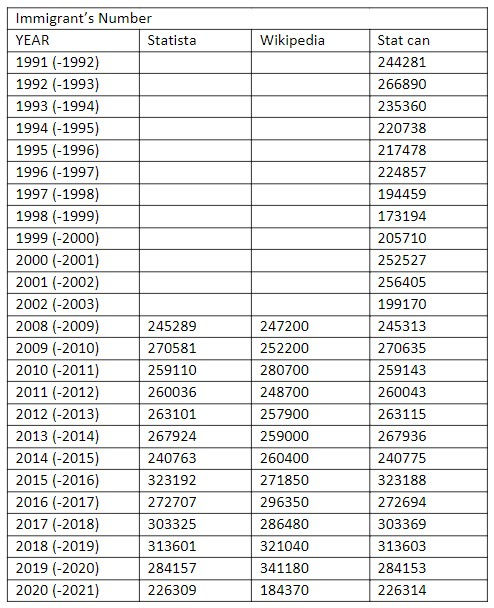
\includegraphics[width= 9 cm]{immigrantsNumber.png}

\includegraphics[width= 12 cm]{TopPlacesOfBirthImmigrants.png}

\includegraphics[width= 12 cm]{TopPlacesOfBirthRecentImmigrants.png}

See Wikipedia.

This shows that a significant proportion of Canada’s recent immigrants are from TB high-incidence countries, e.g. India \cite{Varshney2023TrendsPandemic}, China \cite{Yu2020Estimating2025-2050}, and Philippines\cite{Capeding2022Cost2017}.

Kezia: \url{https://data.worldbank.org/indicator/SH.TBS.INCD?end=2022&locations=AF-CN-CA-AR&start=2000&view=chart}; discuss how we use this website to 

The World Bank, maintains a database of tuberculosis incidence records for each country from the year 2000. We use this tuberculosis incidence data to assign the origin countries where Canada's immigrants come from to either the TB low-incidence countries or the TB high-incidence countries group. Through the labelling and grouping of these countries, we get to observe the trends of tuberculosis numbers in Canada coming from the foreign-born.


\subsection{Data about TB in Canada}

Document time-period of each data.  Data I'm aware of:

\hl{Action item}
\begin{enumerate}
    \item Incidence and prevalence among Canadian foreign-born population 
    \item Total immigration numbers into Canada
    \item Immigrants by continent
    \item Immigrants by country
    \item TB incidence in countries and continents
\end{enumerate}

We have prevalence and incidence.  Carefully cite where data comes from.

\begin{figure}
    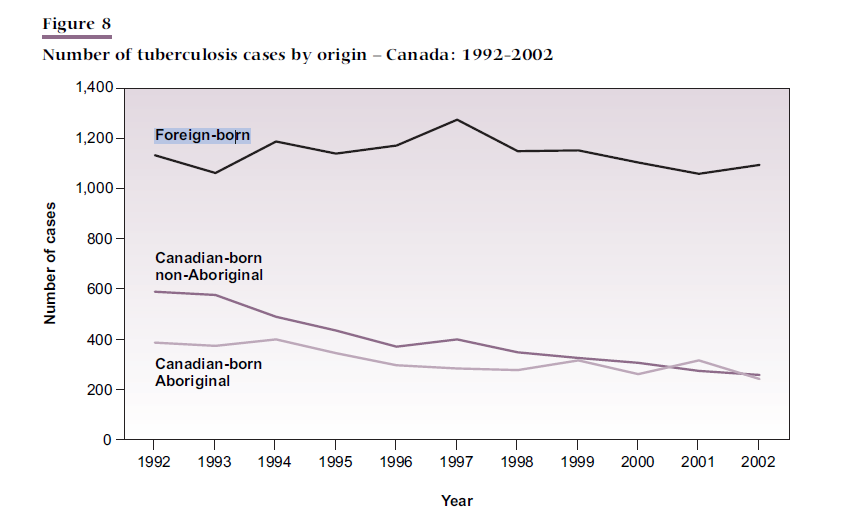
\includegraphics[width=5cm]{IncidencePrevalence1992}
\end{figure}



\subsection{[TIM] Total active tuberculosis cases among Canadian foreign born 1992-2002} 

 \includegraphics[width= 12 cm]{TIM Literature Uploads/Tvs.t.png}

 (Varughese et al, 2014) \url{https://www.researchgate.net/publication/261138130_Preventing_tuberculosis_in_the_foreign-born_population_of_Canada_A_mathematical_modelling_study}



\section{Mathematical Formulation}

\citet{Guo2011PersistentLatency} present a sophisticated compartmental model for the spread of tuberculosis (TB) within the foreign-born population\footnotemark of Canada. We adopt the structure of their model, but update their parameter values based on more current data. In this section, we first present the model of \citeauthor{Guo2011PersistentLatency}, then give our updated parameter values. We were unable to locate reasonable values for some parameters. We discuss our approach to these unknown parameters in Section \ref{sec:data_pars}.

\footnotetext{Depending on the source, there may or may not be a difference between the terms ``foreign-born'' and ``immigrant''. In practice, the operational definition must be checked for each source, regardless of which term is used. In this work, we use the terms interchangeably, and define them both to mean ``something'' (\hl{we need to be careful and precise about this definition. We may actually not be able to get away with a single definition, in which case we can mention the inconsistency of what is being measured as a limitation of our study in the Discussion section}).}

The model used in \cite{Guo2011PersistentLatency} to model TB transmission divides people into five compartments based on their disease status: Susceptible ($\cX$), Early Latent ($\cE$), Late Latent ($\cL$), Active ($\cT$) and Recovered ($\cR$). In brief, individuals begin their life susceptible. A person may become infected upon contact with an active TB case. Immediately after infection, an individual moves to the early latent stage \hl{(the \textit{latent period} is defined as time from infection to infectiousness\cite{InfectiousHandbook})}. From here, they may progress either to late latent or to active TB. After entering the late latent stage, individuals move to active infection after some time. Finally, active cases progress to recovered. 



Discuss $E$ vs $L$.  $E$ means 2 years, not ``before TB becomes dormant." Cite standards 7th edition.

Our model also incorporates demography. That is, individuals can be born (enter the system) and die (leave the system). In our case, birth corresponds to immigration, while death is interpreted literally. We assume that an immigrant may be susceptible or latent, but that the immigration screening process excludes all active cases. We also allow for individuals in any compartment to die, and assume each compartment's death rate is the same (aside for the Active $T$ compartment, which has an additional death-rate to model death due to TB).

\subsection{Equations}

[awk] All the assumptions give rise to the following system of differential equations.

\begin{equation}
    \begin{cases}
        X' &= (1-q_1-q_2)\pi - \beta X \cT - d_X X, \\
        E' &= q_1 \pi + \beta XT - (d_e+\omega)E,\\
        L' &= q_2 \pi + (1-p)\omega E - (d_L + \nu) L,\\
        T' &= pwE + \nu L -(d_T+\alpha+\delta) T \\
        R' &= dT - d_R R
    \end{cases}
    \label{eq:model}
\end{equation}

Figure \ref{fig:flow} gives a diagram of our compartments, along with arrows and rates for all possible transitions. Table \ref{tab:pars} gives more detail on each of the parameters in our model, and Table \ref{tab:init} gives the initial conditions used for our model. Note that some parameters and initial conditions are pulled from the literature, while others are estimated from the data.

\begin{figure}[tpb]
    \centering
    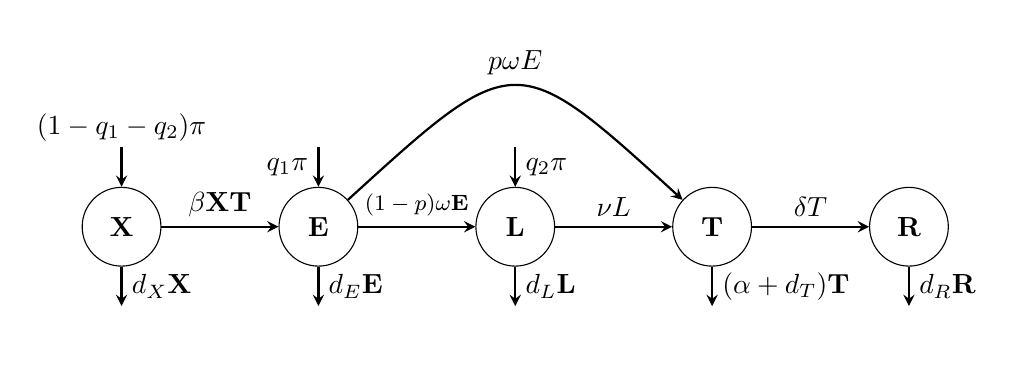
\begin{tikzpicture}[node distance = 2.5cm]
        \node (X) [compartment] {$\cX$};
        \node (E) [compartment, right of=X] {$\cE$};
        \node (L) [compartment, right of=E] {$\cL$};
        \node (T) [compartment, right of=L] {$\cT$};
        \node (R) [compartment, right of=T] {$\cR$};
        \draw [arrow] (X) --  node[align=center, above] {$\beta \cX \cT$} (E);
        \draw [arrow] (E) -- node[align=center, above] {\color{black} \footnotesize $(1 - p) \omega \cE$} (L); % May need to adjust size for final version
        \draw [arrow] (L) -- node[align=center, above] {$\nu L$} (T);
        \draw [arrow] (T) -- node[align=center, above] {$\delta T$} (R);
        % Invisible nodes above and below each compartment for birth/death rates
        \node (aX) [hidden, above=0.5cm of X] {};
        \node (aE) [hidden, above=0.5cm of E] {};
        \node (aL) [hidden, above=0.5cm of L] {};
        \node (bX) [hidden, below=0.5cm of X] {};
        \node (bE) [hidden, below=0.5cm of E] {};
        \node (bL) [hidden, below=0.5cm of L] {};
        \node (bT) [hidden, below=0.5cm of T] {};
        \node (bR) [hidden, below=0.5cm of R] {};
        % Arrows representing birth and death
        \draw [arrow] (aX) node[align=center] {$(1 - q_1 - q_2) \pi$} --  (X);
        \draw [arrow] (aE) -- node[align=center, left] {$q_1 \pi$} (E);
        \draw [arrow] (aL) -- node[align=center, right] {$q_2 \pi$} (L);
        \draw [arrow] (X) -- node[align=center, right] {$d_X \cX$} (bX);
        \draw [arrow] (E) -- node[align=center, right] {$d_E \cE$} (bE);
        \draw [arrow] (L) -- node[align=center, right] {$d_L \cL$} (bL);
        \draw [arrow] (T) -- node[align=center, right] {$( \alpha+d_T ) \cT$} (bT);
        \draw [arrow] (R) -- node[align=center, right] {$d_R \cR$} (bR);
        % Arrow representing skipping the late latent stage (i.e. from E to T)
        \node (aaL) [hidden, above=0.5cm of aL] {}; % Invisible node for jumping high enough above L
        \draw [arrow] (E) .. node[align=center, above] {$p \omega E$} controls (aaL) .. (T);
        
    \end{tikzpicture}
    \caption{Flow diagram for our model of TB transmission.}
    \label{fig:flow}
\end{figure}



\subsection{Finding parameter values}

Include table here.  Then discuss how we found individual parameters, and what they physically / biologically represent.







\begin{table}
    \centering
    \begin{tabular}{ccc}
        Parameter & Description & Value \\
        \hline
        $\pi$ & Annual Immigration Rate & reported \cite{https://www150.statcan.gc.ca/n1/pub/11-630-x/11-630-x2016006-eng.htm}\\
        $q_1$ & Proportion of Early Latent Cases Among Immigrants & Estimated \\
        $q_2$ & Proportion of Late Latent Cases Among Immigrants & Estimated \\
        $\beta$ & TB Transmission Rate & \\
        $d_C$ & Death Rate for Compartment $\mathbf{C}$ & \\
        $\omega$ & Rate of Progressing Past Early Latent Stage & \\
        $p$ & Fraction of Cases Which Skip Late Latent Stage &\\
        $v$ & Rate of Progressing Past Late Latent Stage &\\
        $\delta$ & Recovery Rate from Active TB&
    \end{tabular}
    \caption{Parameters of our model, as well as their specified values and corresponding references. Parameters for which we were unable to find suitable references are labelled as ``estimated''.}
    \label{tab:pars}
\end{table}

\begin{table}
    \centering
    \begin{tabular}{ccc}
    Compartment & Description & Value\\
    \hline
    $\cX_0$ & Susceptible & \\
    $\cE_0$ & Early Latent & Estimated\\
    $\cL_0$ & Late Latent & Estimated\\
    $\cT_0$ & Active TB & Reported \\
    $\cR_0$ & Recovered & 
    \end{tabular}
    \caption{Initial conditions for compartment sizes (i.e. size in 2010). Values are either given (with references) or are labelled as ``estimated''.}
    \label{tab:init}
\end{table}

\subsubsection{Infectivity $\beta$}

 \cite{Guo2011PersistentLatency} use $\beta=1\times 10^{-8}$, while \cite{Ziv2001EarlyInfection} use $\beta=7\times 10^{-6}$.

\url{https://doi.org/10.1201/9781315222912 } ``Infectiousness is dependent on not only the quantity of pathogen in an infected individual, but the ability of the infected host to transmit the pathogen to others.  For example, it is widely accepted that extrapulmonary tuberculosis, unlike its pulmonary form, is not transmissible from an infected host because there is no mechanism for transmission."  \hl{I'd like to cite ch5:} \url{https://www.taylorfrancis.com/chapters/edit/10.1201/9781315222912-5/key-parameters-infectious-disease-epidemiology-laura-white?context=ubx&refId=b6eefe9b-286e-4db4-8740-bebe5eccbf75}

\subsubsection{Latent Tuberculosis}

From \url{https://doi.org/10.1201/9781315222912 } \hl{I'm having difficulty citing this.  I want to cite ch5 from Laura White.}:  The \textit{latent period} of an infectious disease is defined as time from infection to infectiousness, which is slightly different from the \textit{incubation period} (time from infection until onset of symptoms).


Parameters that relate to the $E$ and $L$ compartment.  $q_1,~q_2,~p,~\omega,~\nu$.  



\cite{Ziv2001EarlyInfection} uses $\nu = 0.00256$, which corresponds to 5 percent probability of development of disease over 20 years during the long-term LTBI stage.  




Many TB infections remain latent and never develop to active TB -- \cite{Khajanchi2018DynamicsReactivation} estimate only 5-10\% of latently infected individuals develop active TB.  

\cite{Brooks-Pollock2011}: ``The mean waiting time between first and second diagnoses in households with $\leq$7 adults was 3.5 years, and the distribution was skewed toward shorter times, with a median interval between cases of 1.65 years" 

Newly infected patients ($\leq2$ years from infection) are $15\times$ more likely to develop active TB than people with no known risk factor \cite{PublicHealthAgencyofCanada2014CanadianStandards.} (note the 2022 Standards \cite{Campbell2022ChapterInfection} do not report this number ; hence we use the 2014 Standards \cite{PublicHealthAgencyofCanada2014CanadianStandards.} reported number).  Thus $$ p\omega = 15 \cdot \nu  $$

\cite{Jacquet2006} report $p=5\%$, with a range of $2\%-15\%$.

I'm not sure if $pwE$ flowing into $T$ contradicts $w=0.40$, ``all LTBI immigrants pass through latent stage in the first 2.5 years."

\hl{Ask Will and Albert about this}.  \cite{Ziv2001} states all LTBI immigrants pass through latent stage in the first 2.5 years, which gives a progression rate of $\frac{1}{2.5}=0.40$ people per year.  This will give an exponentially distributed rate of progression (?) where on average, an infected will leave the $E$ compartment in 2.5 years.  However, in practice, people in $E$ do not leave at an exponential rate.  This could be fixed by using more compartments for $E$ (source?).

% Immigrant population data - Statistics Canada.
% $$ ReportedTB = [14.6 14.4 14.1 14.7 14.6 15 14.3 15 15.5 15 14.8 15.9 14.3]$$ %Actual TB rate from 2008 - 2020


% Incident rate data

%Parameter values for simulations of the compartmental TB model (1) with early and late latently-infected new immigrants.


\section{Numerics}

I have difficulty splitting this section into smaller sections.  

How we did the code:
\begin{itemize}
    \item Data: incidence data.
    \item Setting up objective function and constraints.
    \item Finding initial conditions (via steady state).
    \item Numerically verifying our solution is minimum.  KKT conditions.
    \item Preconditioning by rescaling. 
\end{itemize}

Analyzing results:
\begin{itemize}
    \item Sensitivity analysis.
    \item Histograms.
    \item Sniff test?  Compare to other sources.
\end{itemize}

\subsection{Estimation}
\label{sec:estimation}
\hl{Citations needed for methodology. I have some I can use for optimization, but it's worth looking into how Matlab likes to be cited.}

We begin with the estimated parameters, $q_1$, $q_2$, $\cE_0$ and $\cL_0$. For fixed values of the non-estimated parameters, we estimate $q_1$, $q_2$, $\cE_0$ and $\cL_0$ my minimizing the least-squares error for the observed incidence rate of TB among foreign-born individuals in Canada between the years of \hl{2010 and 2020 (confirm this)}. More precisely, for particular values of the non-estimated parameters, we use the \texttt{ode23} function in \texttt{Matlab} \hl{(citation for Matlab? for ode23? I have inserted the citation here; is this what you want?)} \cite{TheMathWorksInc.2022MATLABR2022b} to solve System \ref{eq:model}. This solution consists of trajectories for the sizes of the compartments in our model. We then compute the TB incidence at each time point using the expression in \citet{Guo2011PersistentLatency}: $pwE +vL$. Our objective function is the squared $\mathcal{L}^2$ difference between predicted and observed incidence at each time point where we have data (\hl{normalization?}). 

Optimization is performed using the \texttt{fmincon} function in \texttt{Matlab}. This function iteratively attempts to take a ``direct step'', in which the KKT equations are approximated using the finite difference method, then linearized and solved. Alternatively, if the Hessian obtained from the finite difference method is not positive definite, the Conjugate Gradient method is used instead for the current iteration.

Figure ??? gives the observed incidence trajectory, as well as our estimated incidence trajectory after optimizing $q_1$, $q_2$, $\cE_0$ and $\cL_0$, where we have used values from \citet{Guo2011PersistentLatency} for the non-estimated parameters. For reference, we also include the estimated incidence trajectory obtained by using values from \citet{Guo2011PersistentLatency} for the estimated parameters. Note that optimizing parameters here improves the fit dramatically.

\subsection{Analysis}

\hl{This section got moved and may need to be rearranged.}


The parameters of our model are broadly divided into two groups: those obtained from the literature, and those we estimate. Our analysis treats these groups separately. We begin by fixing all unestimated parameters at plausible values. We then optimize over the estimated parameters, calibrating our model to match observed TB incidence. Finally, we investigate sensitivity to our choices of unestimated parameter values by repeating the above process with several different values for each unestimated parameter (\hl{awk}) \cite{Razavi2021TheSupport}. In this section, we describe our treatment of the unestimated and unestimated parameters in more detail, and discuss what outputs we extract from our individual simulations and sensitivity analysis.

\subsection{[Will] Sensitivity}

Those parameters not estimated (i.e. all except $q_1$, $q_2$, $\cE_0$ and $\cL_0$) are fixed at levels determined from the medical and epidemiological literature. In order to explore the impact of these parameters on the overall model, we select a range of values for each and repeat the analysis described in Section \ref{sec:estimation} at every combination of parameter values. This gives us a measure of how sensitive our findings are to each parameter over the range of values we explore. For more on sensitivity analysis, see Razavi et al \cite{Razavi2021TheSupport}. 

[awk] Each non-estimated parameter has either three or four levels (see Tables \ref{tab:pars} and \ref{tab:init}), and there are a total of \hl{???} combinations. For each such parameter, we divide all analyses based on the levels of that parameter. We then plot all incidence trajectories obtained from a single level of that parameter in the same plot, along with the average trajectory. We then plot the average trajectory for each level of the parameter, as well as the global average trajectory. This combination of plots gives a visual representation of the relative variability of estimated incidence across levels of the parameter. Comparing plots across parameters allows us to assess the relative sensitivity of our model to each non-estimated parameter.

In addition to the above trajectory plots, we also investigate the distribution of parameter estimates across all configurations of the non-estimated parameters. Figure \ref{fig:est_dist} gives a histogram for our final estimates of each of $q_1$, $q_2$, $E_0$, $L_0$ and $R_0$. These histograms display the range of values for each parameter. Recall that $\cL_0$ is minimally affected by optimization, so the three bars in its histogram correspond to the three initial values for this parameter. \hl{Is next sentence a typo?} In order to see how well fitted models match the available data, we also give a histogram of the optimal objective function value achieved under each configuration of the non-estimated parameters. See Figure \ref{fig:err_dist}.







While it is instructive to investigate the breadth of our parameter estimates, we are mostly interested in the best such estimates. To this end, we restrict attention to the \hl{3? 5?} parameter estimates that most closely match our dataset (i.e. with smallest optimal objective function value). These ``best'' estimates are shown in Figure \ref{fig:est_dist} by vertical lines. The difference in objective function between the first and \hl{(third? fifth?} best estimates is negligible \hl{(confirm this)}.


\subsection{Defining the loss function}

Using Matlab's \texttt{ode23} routine, we solve the system of differential equations from \cite{Guo2011PersistentLatency}, which returns population vs time.  From the population, we compute the incidence estimated TB incidence $\hat{f}(t)$
  	$$\text{Estimated TB Incidence } = \frac{100,000}{X(t)+E(t)+L(t)+T(t)+R(t)} \cdot (pw E(t) + v L(t)) ,$$
which can be compared to the reported TB incidence in from official Canadian reports $f(t)$\cite{MounchiliA.2022TuberculosisReport}.  Our loss function is defined to be the difference between our computed (estimated) incidence and the reported incidence,
 $$ \text{Error = } \int_{2010}^{2020} (\hat{f}(t) - f(t))^2 dt. $$
\hl{In practice, $f(t)$ is reported annually from 2010 to 2020, and so we compute $\hat{f}(t)$ discretely. [awk]} 


\subsection{Specifying initial conditions}

To solve the system of differential equations, initial conditions $[X_0, E_0, L_0, T_0, R_0]$ are required, which correspond to the foreign-born population distribution in 2010.  $T_0$ is reported to be 1054 \cite{MounchiliA.2022TuberculosisReport}, and the total foreign-born population is reported to be 6516655 (found by taking the Census reported foreign-born population in 2011 and subtracting the immigration rate in 2010)) [\hl{should I round this to 650k?}].

\subsubsection{Including $E_0$ and $L_0$ as parameters in the solver}

The optimizer does not search across $L_0$.  Figure \ref{fig:OptimizedParameterDistribution4param} shows whatever $L_0$ we start at, we essentially stay at. 

\begin{figure}
\centering 
    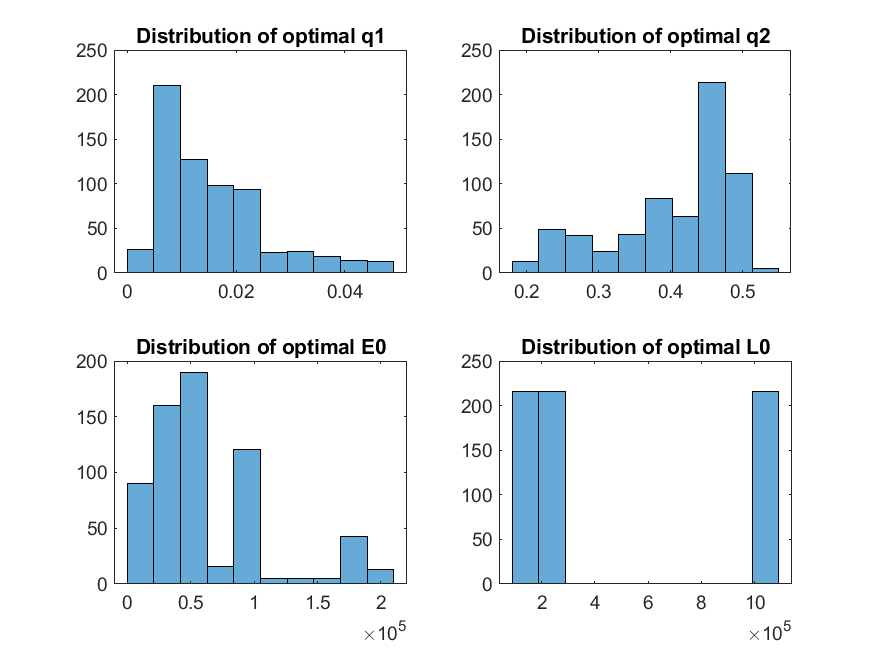
\includegraphics[width=0.8\textwidth]{Optimized parameter distribution across sensitivity analysis.png}


    \caption{After running sensitivity analysis, this is the distribution of the optimized values of $q_1,~q_2,~E_0,~L_0.$  Notice that $L_0$ has a peculiar distribution -- this is because the optimized value of $L_0$ is always very close to the pre-optimized initial choice of $L_0$.}
    \label{fig:OptimizedParameterDistribution4param}
\end{figure}


\subsubsection{Setting $E_0$ and $L_0$ based on incidence}

Recall with $t_0=2010$
  	$$\text{Estimated TB Incidence in 2010} = \frac{100,000}{X(t_0)+E(t_0)+L(t_0)+T(t_0)+R(t_0)} \cdot (pw E(t_0) + v L(t_0)) ,$$
The denominator is exactly the total foreign-born population \hl{QUOTE ABOVE}, and the reported incidence in 2010 is 14.1 \cite{MounchiliA.2022TuberculosisReport}, thus we could choose $E_0$ and $L_0$ so $$\text{Estimated TB Incidence in 2010~} = 14.1. $$
However, this problem is under-determined and has no unique solution.


\subsubsection{Initial conditions with the Point-wise Stationary Approximation}

In queuing theory, the pointwise stationary approximation of a queue system approximates any time of a queue system using its steady state (holding any time-dependent parameters constant) \cite{Whitt1991} \hl{[check with Sandy]}.

We estimate the initial conditions using the steady state of the system of DEs, which has a globally asymptotically stable unique endemic equilibrium \cite{Guo2011PersistentLatency}.  The steady states are found numerically by simulating to steady state.  We have three ways to assess the accuracy of this approximation:
\begin{enumerate}
    \item Compare the steady state's total population to the reported total population.
    \item Compare the steady state's $T_0$, which is reported to be 1054.
    \item Compare the steady state's estimated incidence, which is reported to be 14.1.
\end{enumerate}



\subsection{[Jeremy] Optimization Results}

See Figure \ref{fig:OptimizedResults} to compare pre- and post- optimization behaviour.

\begin{figure}
    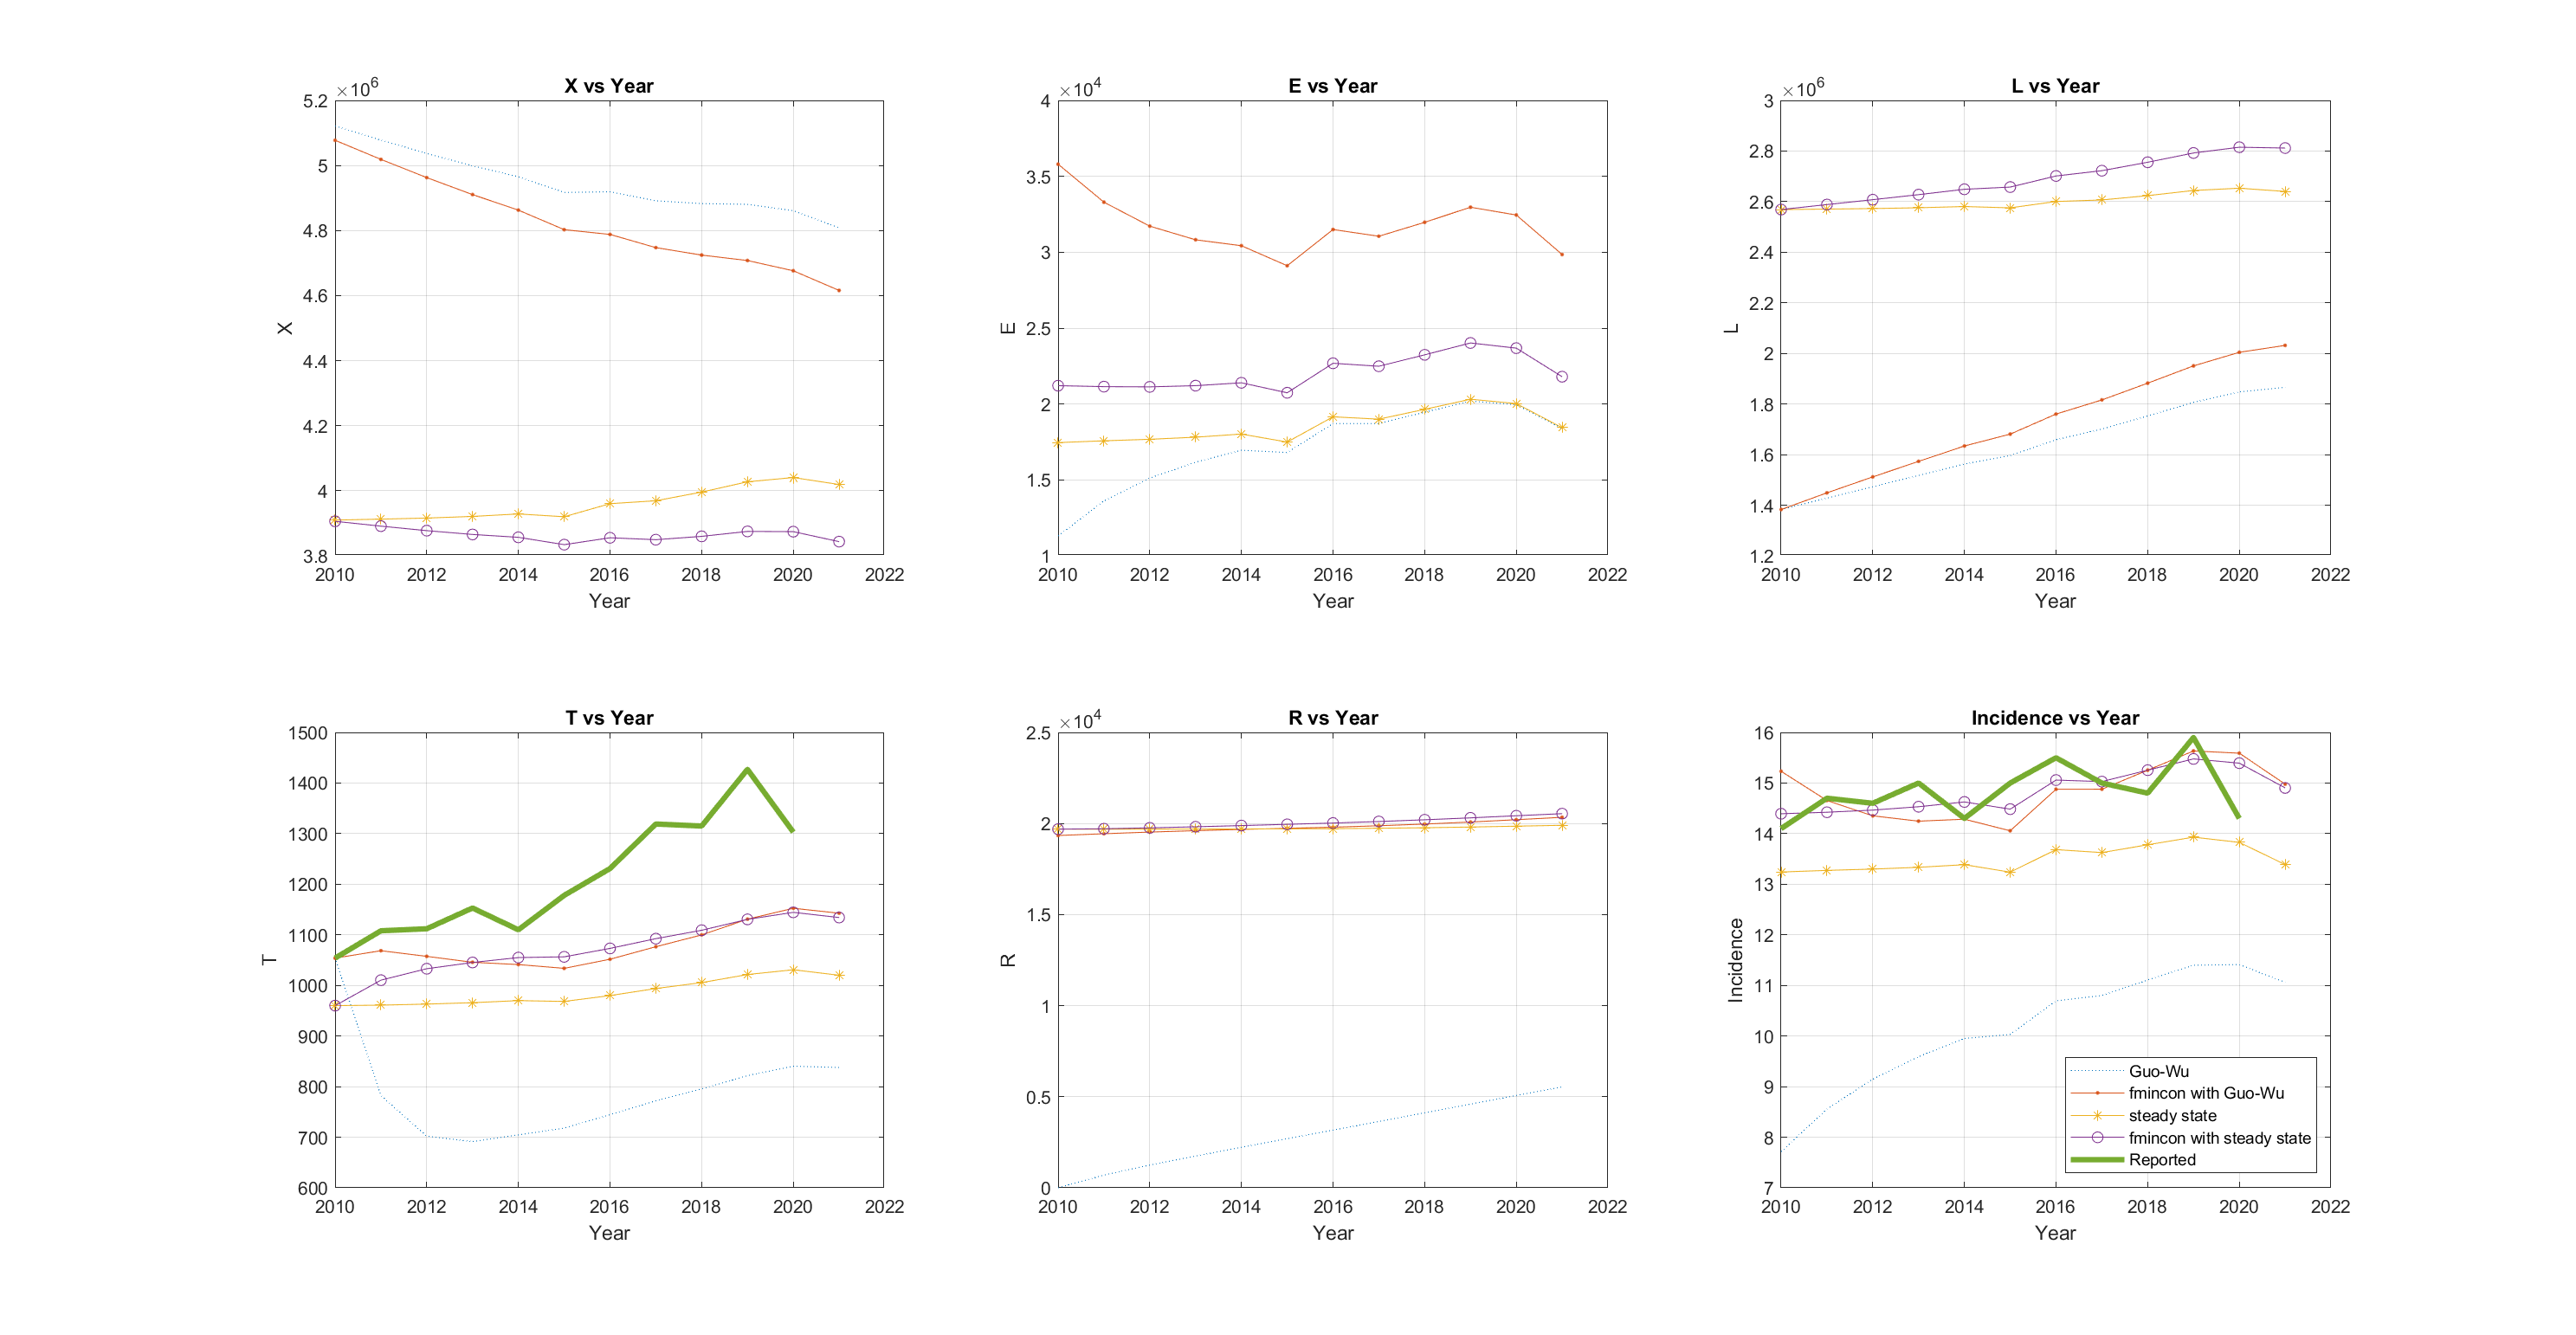
\includegraphics[width=\textwidth]{PopVsTime_various}

    \caption{Graphs of the population vs time, and the incidence vs time.  There are four experiments -- parameters from Guo-Wu\cite{Guo2011PersistentLatency}, \texttt{fmincon}'s optimized parameters with Guo-Wu's parameters as initial conditions, the steady-state, and \texttt{fmincon}'s optimized parameters with steady-state as initial conditions. }
    \label{fig:OptimizedResults}
\end{figure}

\subsection{[Jeremy] Sensitivity Analysis}

We performed sensitivity analysis across several different parameters.  We found that the results are most sensitive to $\nu$, $\omega$, and $L_0$; which is unsurprising since they explicitly appear in the loss function (however, the  is not sensitive to $E_0$).  See figure \ref{fig:SensitivtyBigPlot}.


Figure \ref{fig:OptimizedParamsSensitivity} a distribution of the optimized parameters.  Notice $L_0$ and $R_0$ do not deviate much from their initial value -- this is emphasized in the second plot.  

\begin{figure}
    \centering
    \begin{subfigure}[b]{0.475\textwidth}
    \centering
        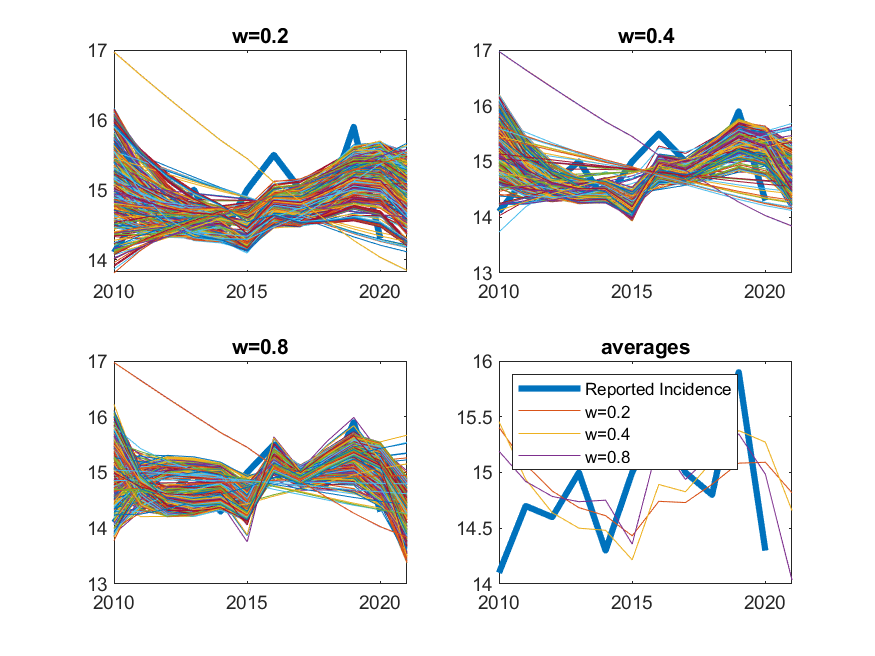
\includegraphics[width=\textwidth]{Sensitivty_w Run 2.png}
    \end{subfigure} 
  \hfill   
    \begin{subfigure}[b]{0.475\textwidth}
    \centering
     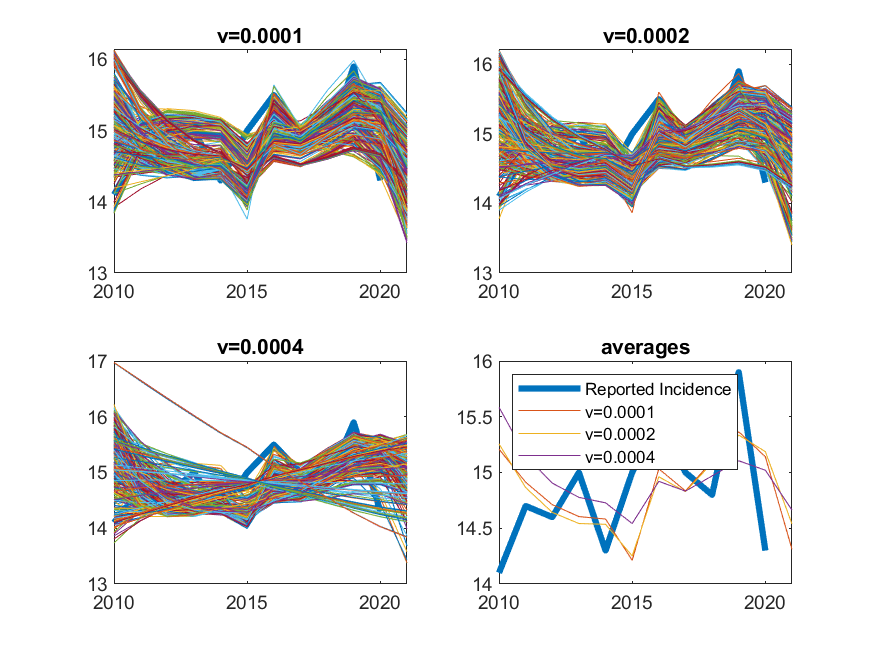
\includegraphics[width=\textwidth]{Sensitivty_v Run 2.png}  
    \end{subfigure} 
            \vskip\baselineskip

    \begin{subfigure}[b]{0.475\textwidth}
    \centering
     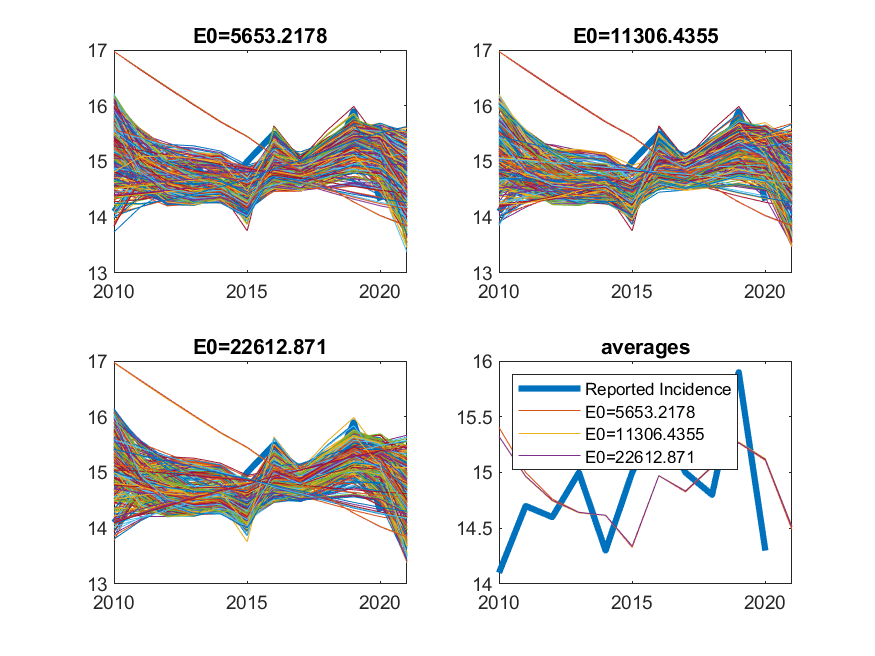
\includegraphics[width=\textwidth]{Sensitivty_E0 Run 2.png}  
    \end{subfigure} 
    \hfill
    \begin{subfigure}[b]{0.475\textwidth}
    \centering
     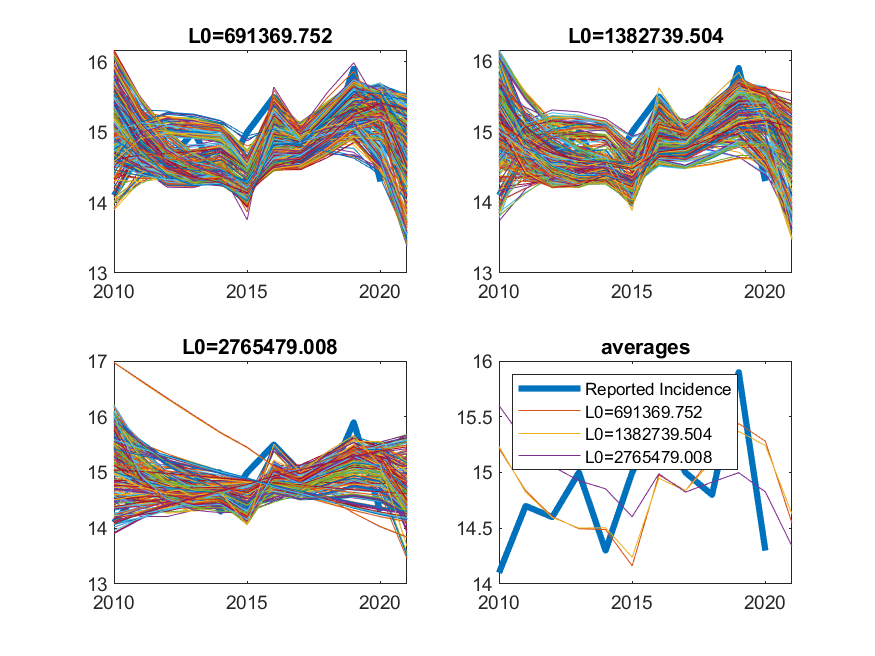
\includegraphics[width=\textwidth]{Sensitivty_L0 Run 2.png}  
    \end{subfigure} 
    
    \caption{Our results were most sensitive across $\nu$, $\omega$, and $L_0$. There is little sensitivity across the choice of initial $E_0$.  In the second figure, the dashed lines are the initial conditions.}
    \label{fig:SensitivtyBigPlot}
\end{figure}

\begin{figure}

    \centering
         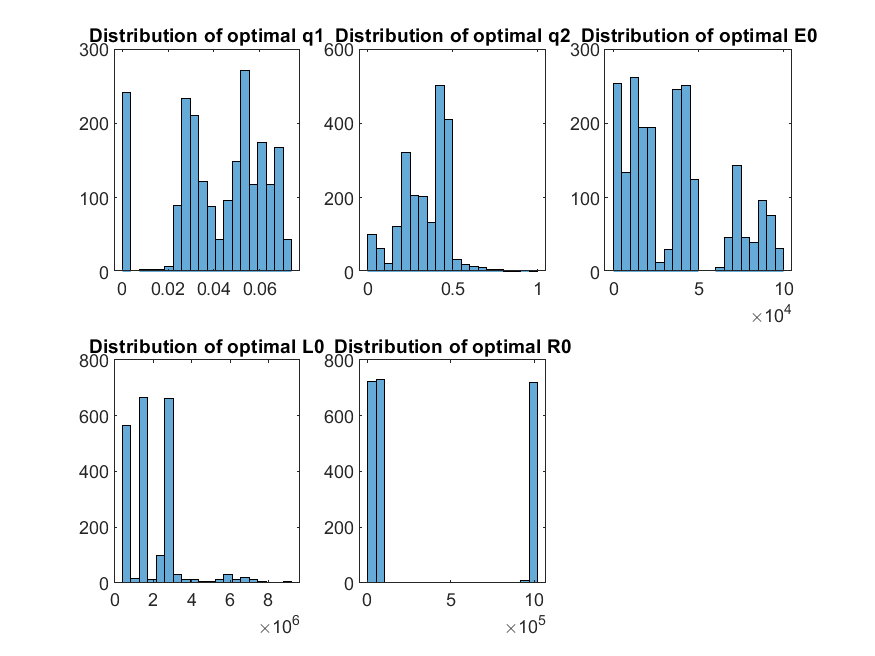
\includegraphics[width=0.8\textwidth]{Optimized parameter distribution across sensitivity analysis Run 2.png}  
         
        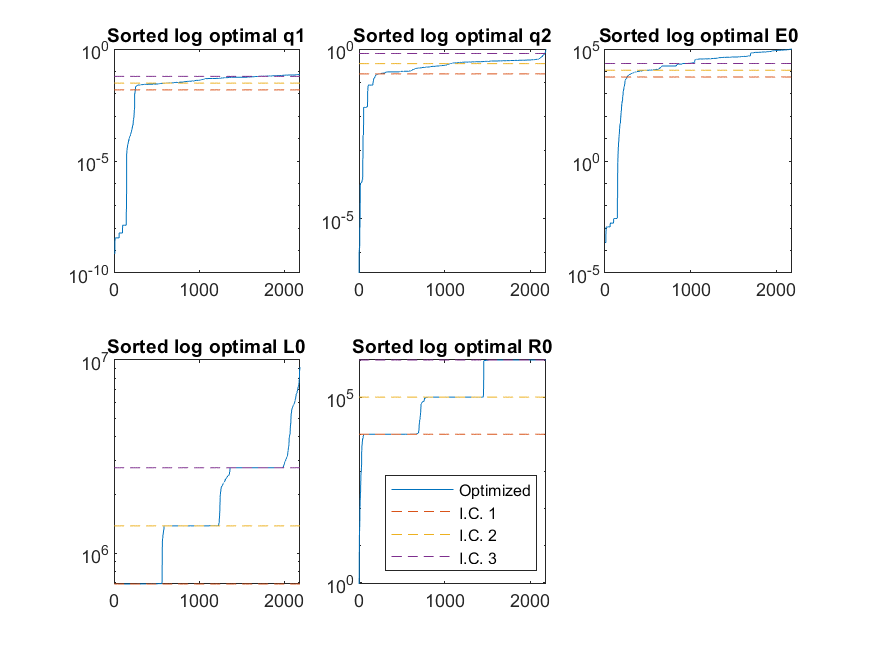
\includegraphics[width=0.8\textwidth]{Optimized parameter log sorted with starting values Run 2.png}
        
    \caption{Historgram of optimized parameters.  Notice the $L_0$ and $R_0$ don't change much from their initial value.  The second plot highlights this -- notice how many of the optimal $L_0$ and $R_0$ are just the initial condition.}
    
    \label{fig:OptimizedParamsSensitivity}
\end{figure}
    

\begin{figure}
    \centering
         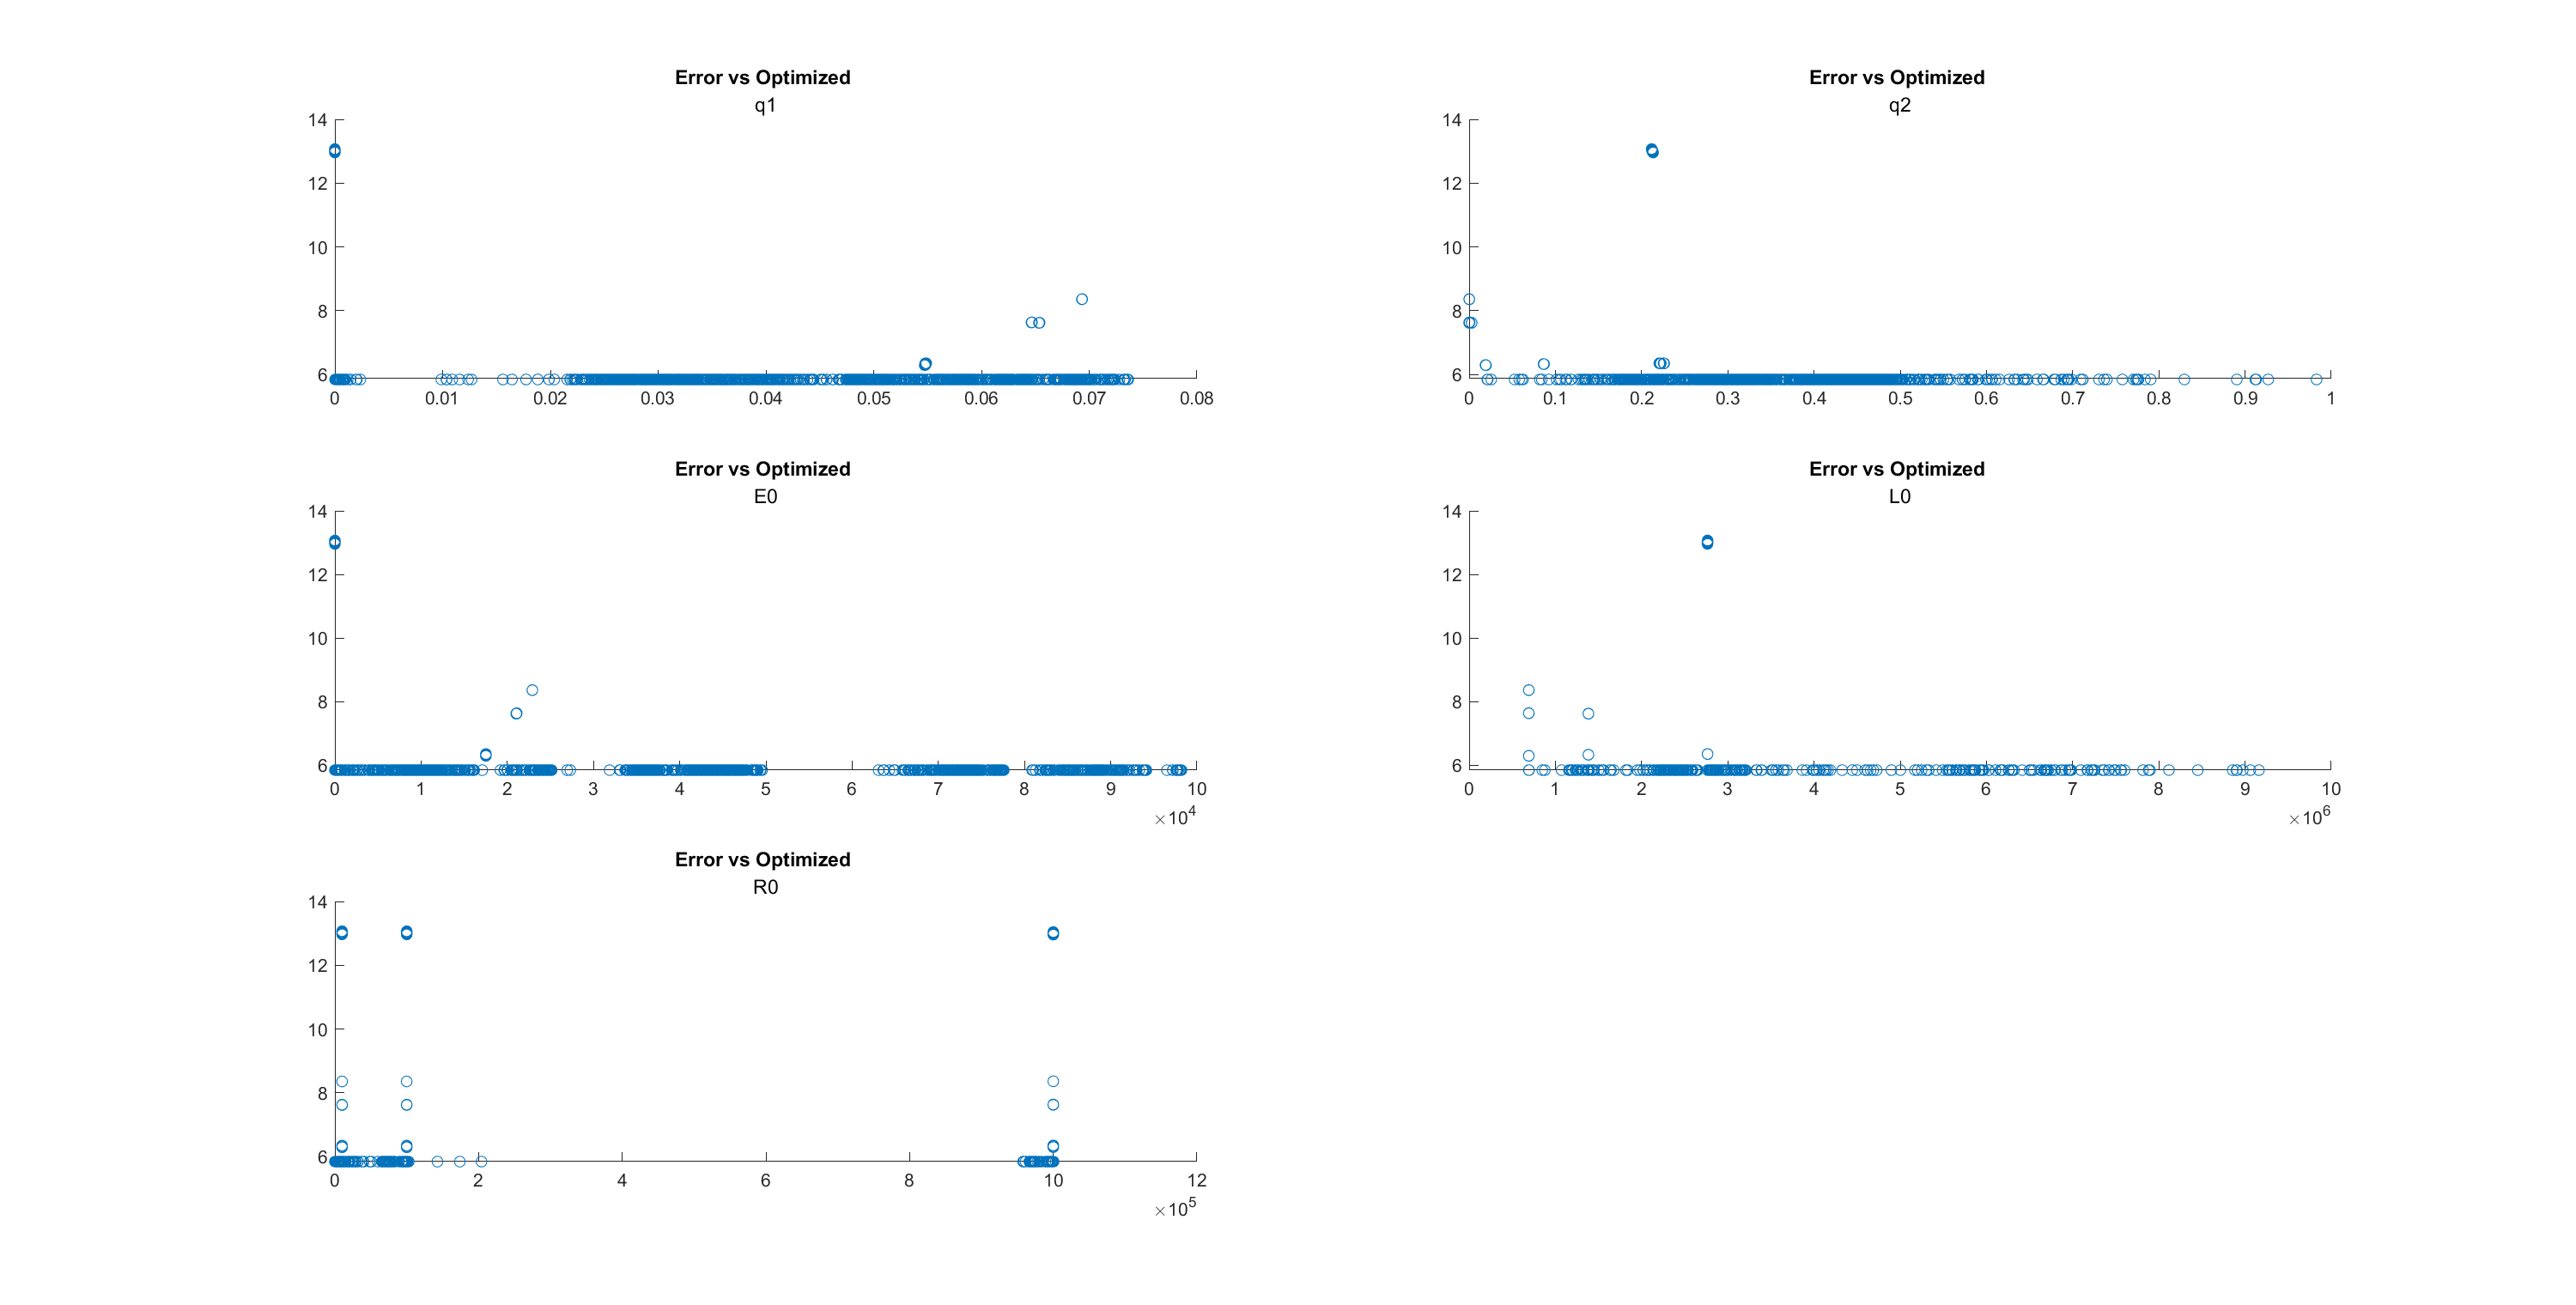
\includegraphics[width=0.8\textwidth]{ScatterPlotErrorVsOptimalOutput Run 2.png}  

         
        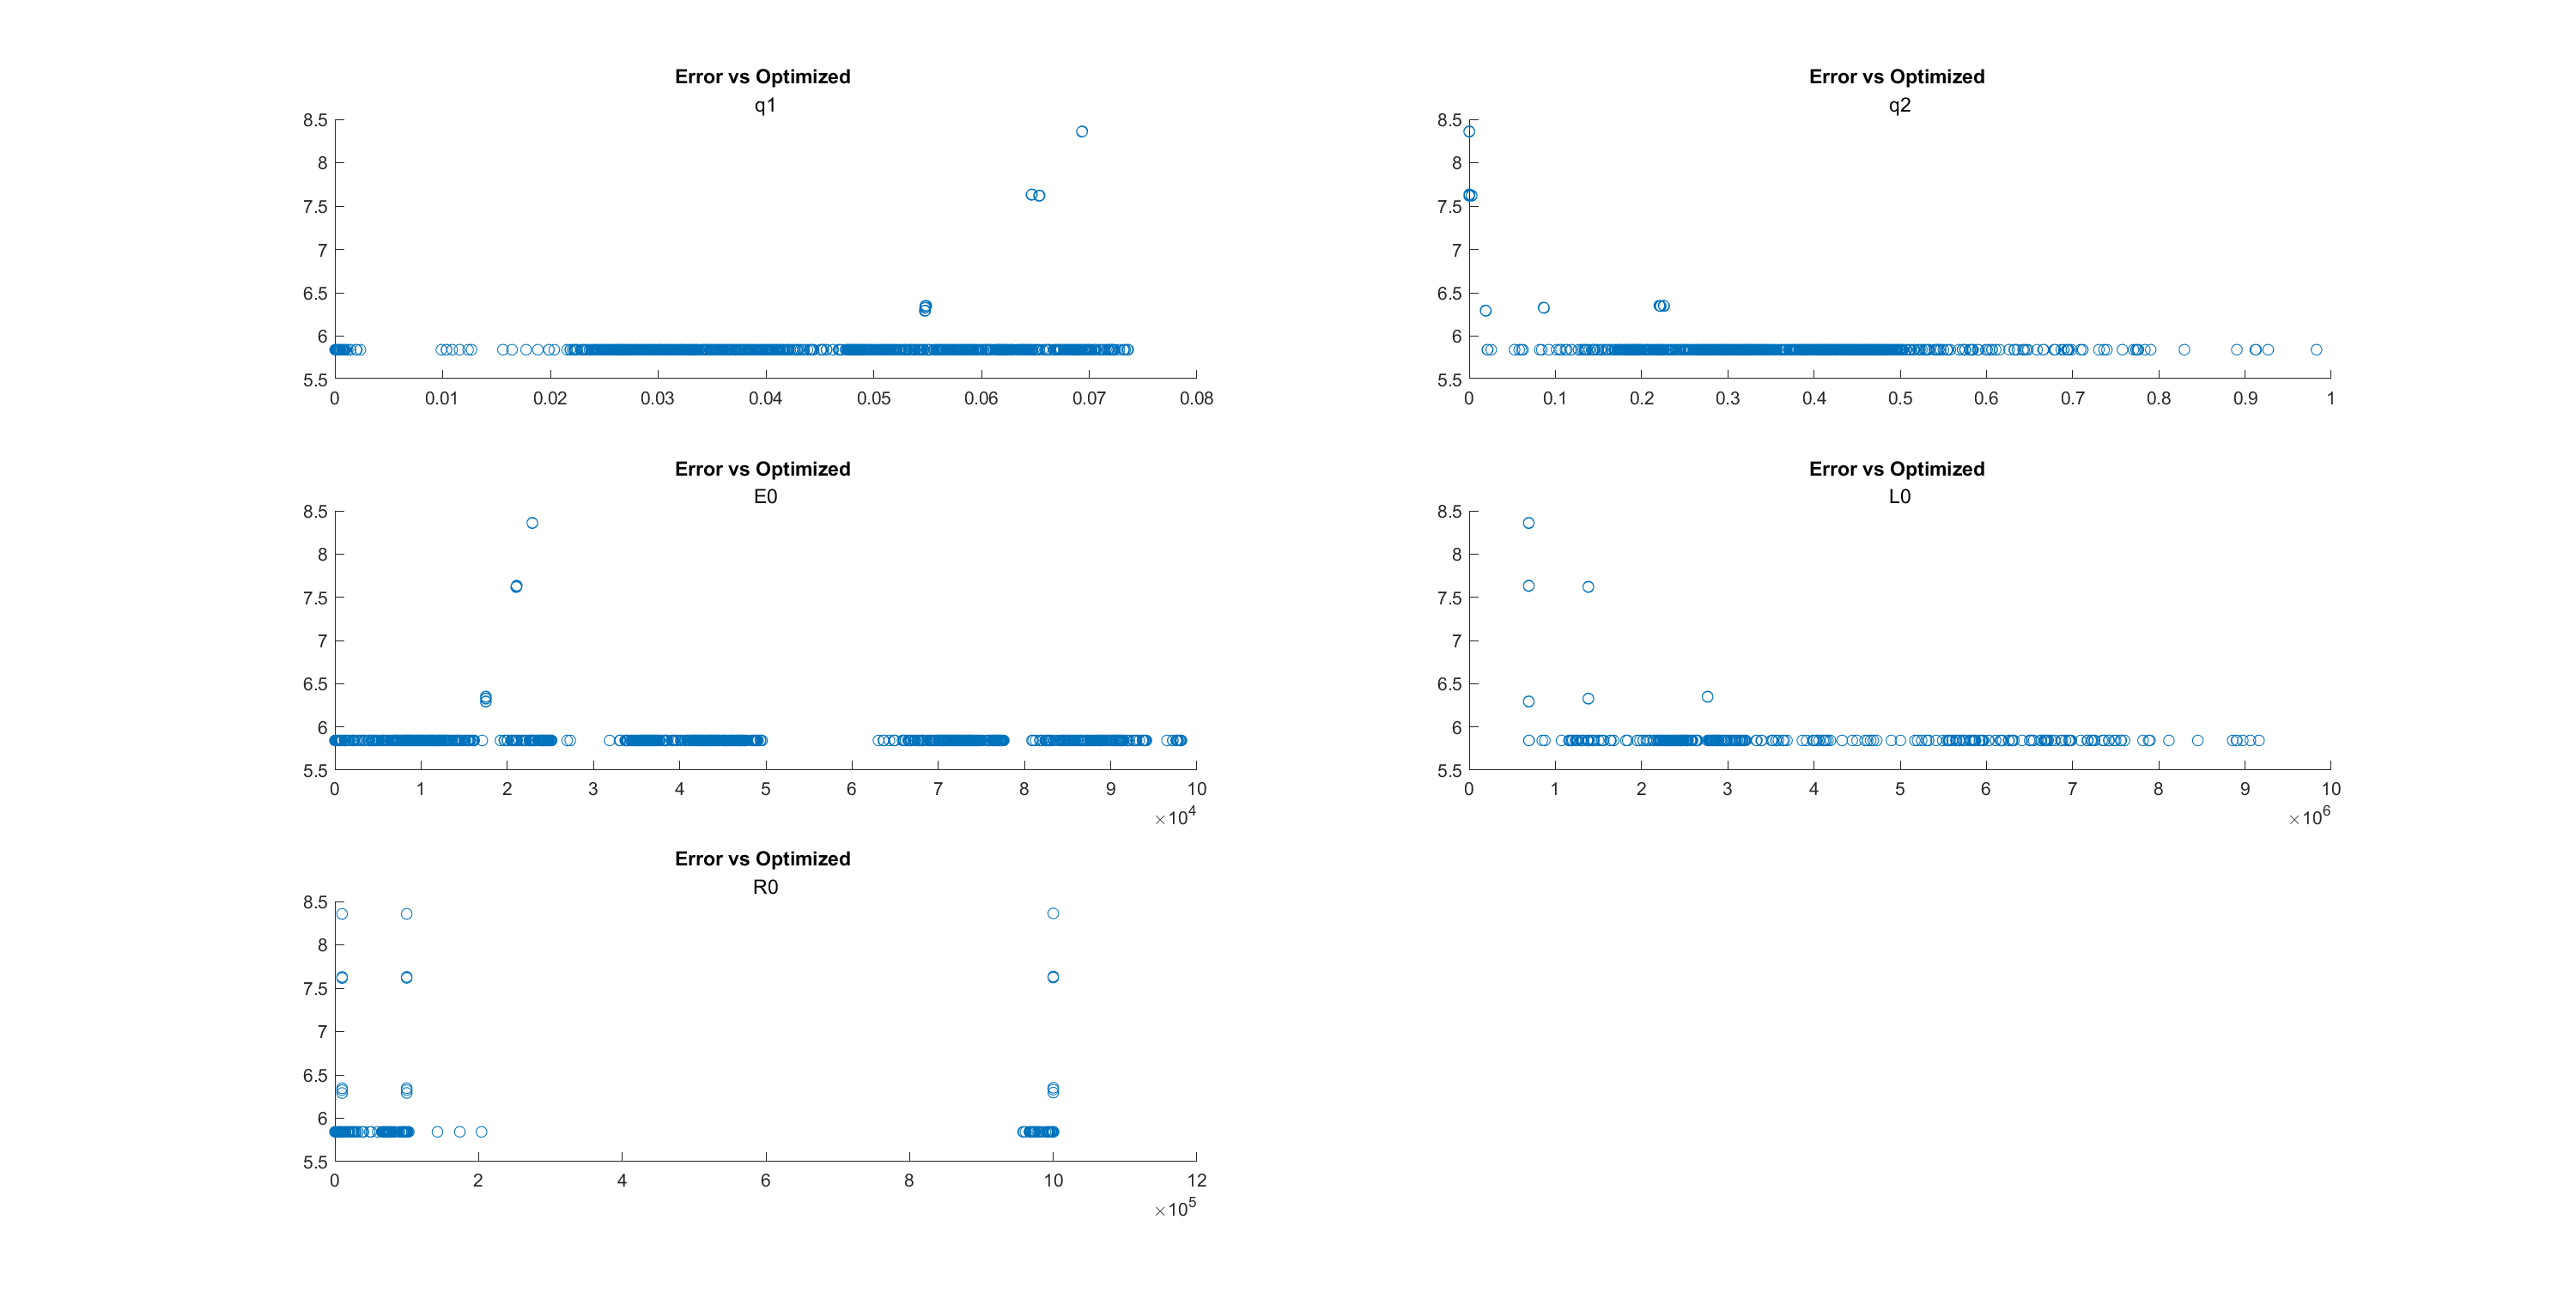
\includegraphics[width=0.8\textwidth]{ScatterPlotErrorVsOptimalOutput_Cut2 Run 2.png}

        \caption{This is a scatter plot of the error vs optimized parameter. As we zoom in and delete outliers, we see more apparent outliers.  ``This is what the tail of a distribution will often look like. It does suggest that the outliers aren't typos"}

        \label{fig:ScatterErrorVsOptimizedParam}
\end{figure}

\section{Optimization and Numerical Analysis}

\subsection{Sensitivity analysis on $\omega$, $\nu$, $q_1$, and $q_2$}

Uses steady state as initial condition.

From earlier investigations, we found our results were most sensitive to $\omega$, $\nu$, $q_1$, and $q_2$.  We picked an initial condition for them, then scaled them by $(0.90).^{[1,0,-1,-2]},$ giving a total of $ 4^4 = 256$ combinations.  See figure \ref{fig:SensitivtyAverages5}, which shows the results are not sensitive to $\omega$, but somewhat sensitive to $\nu$, $q_1$, and $q_2$.  I suspect $\nu$ is the most important because $q_1$ and $q_2$ are thrown into the optimizer anyway.  See figure \ref{fig:SensitivtyAverages5}

\begin{figure}
	\centering
	\begin{subfigure}[b]{0.475\textwidth}
		\centering
		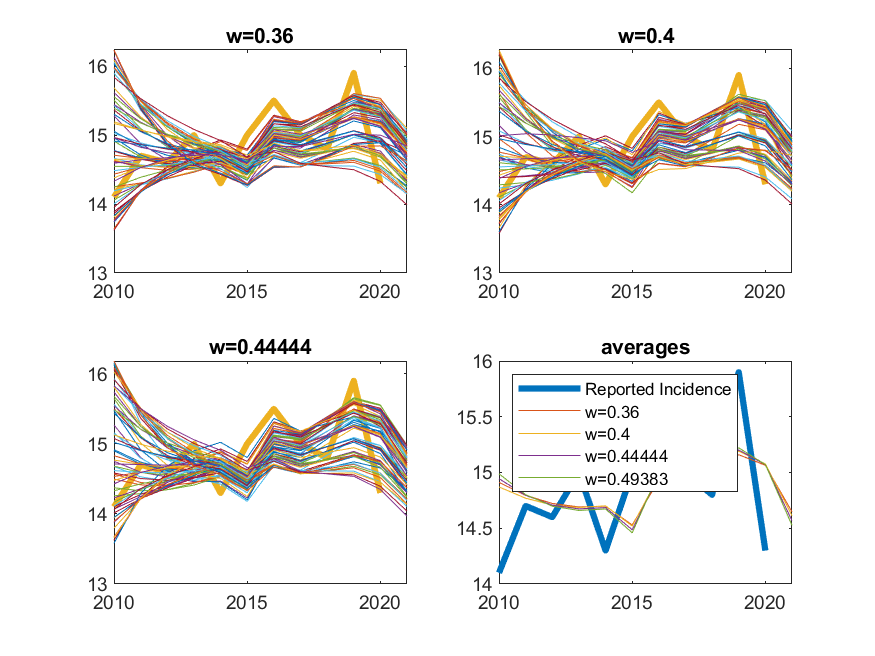
\includegraphics[width=\textwidth]{Sensitivty_wRun5.png}
	\end{subfigure} 
	\hfill   
	\begin{subfigure}[b]{0.475\textwidth}
		\centering
		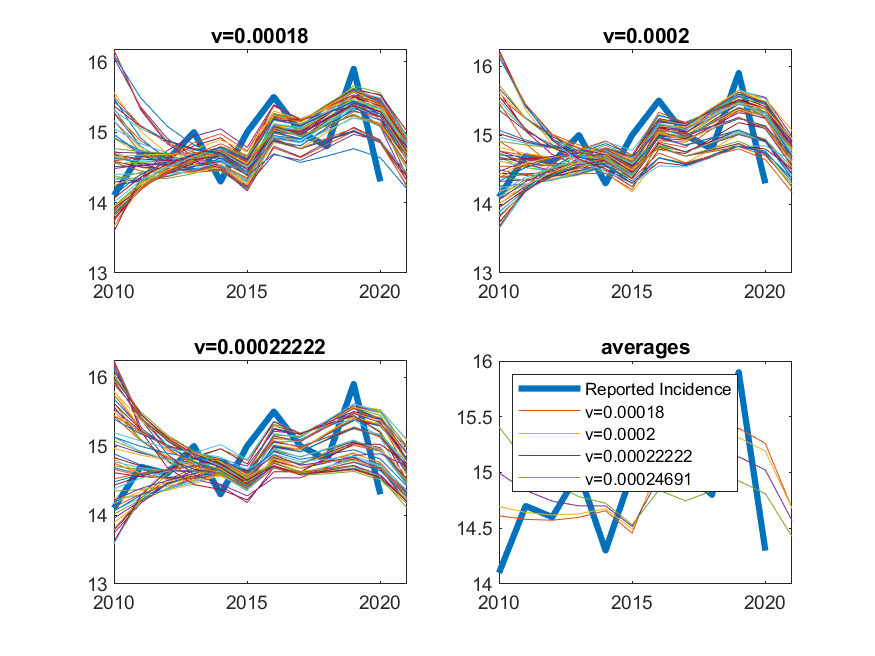
\includegraphics[width=\textwidth]{Sensitivty_vRun5.png}  
	\end{subfigure} 
	\vskip\baselineskip
	
	\begin{subfigure}[b]{0.475\textwidth}
		\centering
		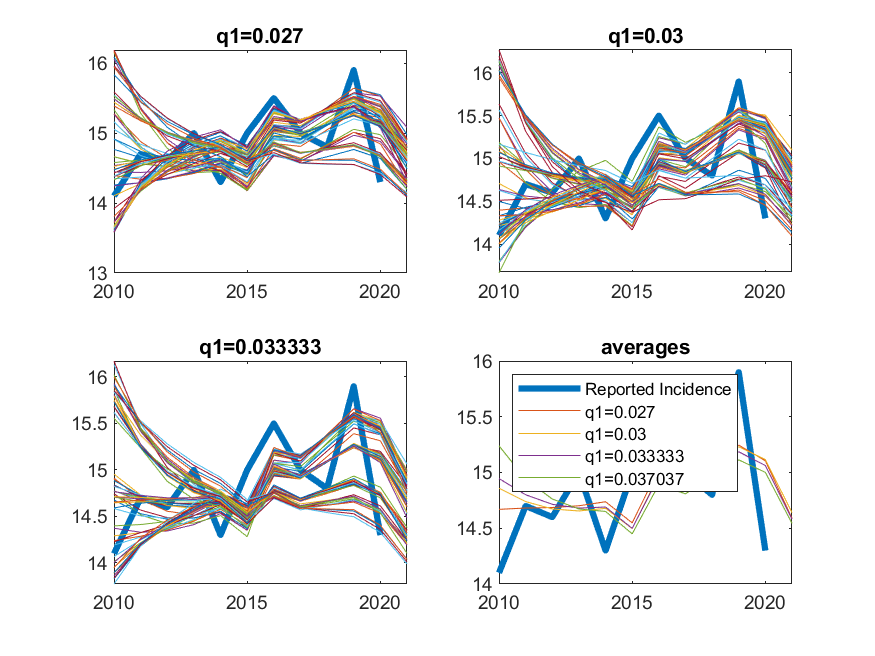
\includegraphics[width=\textwidth]{Sensitivty_q1Run5.png}  
	\end{subfigure} 
	\hfill
	\begin{subfigure}[b]{0.475\textwidth}
		\centering
		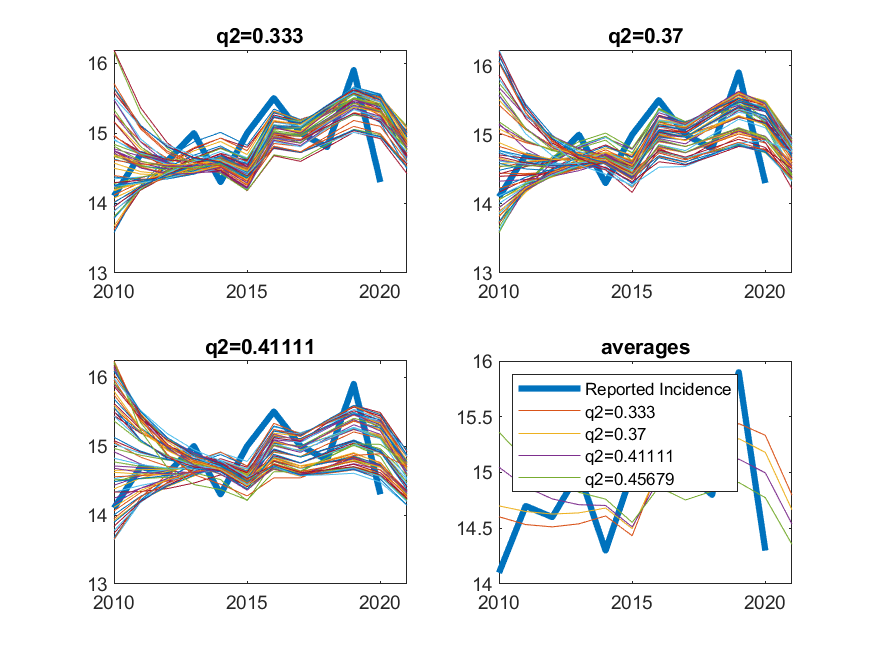
\includegraphics[width=\textwidth]{Sensitivty_q2Run5.png}  
	\end{subfigure} 
	
	\caption{I don't see anything irregular with these results.  The only things I notice is that as $\nu$ gets smaller, the incidence in 2010 improves.}
	\label{fig:SensitivtyAverages5}
\end{figure}

\subsection{Examining \texttt{fmincon} output}

Among the 256 experiments we performed during sensitivity analysis, we look at the set of parameters that minimize and maximize the errors, then examine some of $\texttt{fmincon}$'s outputs.  For the minimizing set, \texttt{fmincon} took 11 iterations with a total function count of 142.  This number is consistent with the fact that \texttt{fmincon} uses central finite differencing; since there are 5 dimensions, each gradient would cost 10 function evaluations (i.e. 110 function evaluations to evaluate the gradient).  Other factors like backtracking could contribute to the remaining 32 evaluations.
%, such as the gradient $\nabla f$ and hessian $H$.

\subsection{Gradient and Hessian - preconditioning. scaling variables} 

We found
$$ \nabla f _{\text{min}} = [4.46e-03,~-1.56e-05,~-3.13e-10,~-7.99e-12,~2.76e-12 ] ,$$ 
and
$$ \nabla f _{\text{max}} = [4.09e-01,~-5.00e-03,~-1.21e-03,~-9.43e-06,~1.35e-09 ] .$$ 
Notice the largest partial derivatives are $f_{q_1}$ and $f_{q_2}$, while $f_{E_0}$, $f_{L_0}$, and $f_{R_0}$ are small.  This is consistent with our sensitivity analysis demonstrating that our model was most sensitive to $q_1$ and $q_2$.

Recall that we expect the gradient to approach zero near a minimum.  Notice that $$\| \nabla f_{\min} \|_\infty = 4.46 e-03 \ll \| \nabla f_{\max} \|_\infty = 4.09 e-01. $$  
$\nabla f_{\max}$ is 100 times larger than $ \nabla f_{\min} $, suggesting the the optimizer should continue searching at the maximum.  It turns out the error-maximizing parameter is poorly conditioned, which is demonstrated by the Hessian $H$.

\subsection{Hessian}

Recall at a local minimum, the Hessian should be symmetric positive definite.  This is numerically verified by computing the eigenvalues of the Hessian matrix.  We found the eigenvalues $\lambda$
$$ \lambda(H_{\min})  = [5.2868e-04,~ 3.2415e-01,~1.0000e+00,~1.0000e+00,~8.4916e+05],$$ 
while
$$ \lambda(H_{\max})  =   [ 2.9168e-09,~1.0000e+00,~1.0000e+00,~1.5888e+02,~1.7682e+08].$$
Although all eigenvalues are positive, the small eigenvalues in $H_{\max}$ are driving the condition number up, which may be causing problems for the optimizer and thus the large gradient.
%So we again do sensitivity analysis

For $H_{\min}$, the eigenvectors are as follows (each column is an eigenvector):

\[
  \begin{bmatrix}
	-0.0314146 & -0.0003089 &  0.0000034 &  0.0000000 & -0.9995064 \cr
	0.9994670 &  0.0088770 & -0.0001204 & -0.0000016 & -0.0314161 \cr
	0.0067183 & -0.7473443 &  0.6637665 & -0.0290771 &  0.0000221 \cr
	-0.0000319 &  0.0044353 &  0.0487478 &  0.9988013 & -0.0000002 \cr
	0.0058115 & -0.6643628 & -0.7463496 &  0.0393770 &  0.0000201
\end{bmatrix}
\]
with respective corresponding eigenvalues 
\[
  \begin{bmatrix}
	0.0005287 &  0.3241506 &  1.0000000 &  1.0000000 & 849155.2834507
\end{bmatrix}
\]

Observe that by far, the largest eigenvalue is the fifth value.  The fifth eigenvector is nearly the basis vector $[-1 ~0~ 0~ 0~ 0]$, which corresponds to $q_1$.  This suggests each variable is on a different order of magnitude, and so we should rescale; see section \ref{subsec:normalization}.

\subsubsection{Taylor Expansion}


Recall the multivariate Taylor expansion of a function $f(x)$ at a point $\vec{a}\in\mathbb{R}^n$:
%
%$$ y = f(\mathbf{x})\approx f(\mathbf{a}) + \nabla f(\mathbf{a})^\mathrm{T} (\mathbf{x}-\mathbf{a}) + \frac{1}{2}(\mathbf{x}-\mathbf{a})^\mathrm{T} \mathbf{H}(\mathbf{a}) (\mathbf{x}-\mathbf{a}) + O( \|\mathbf{x}-\mathbf{a}\|^3). $$

$$ y = f(\vec{x})\approx f(\vec{a}) + \nabla f(\vec{a})^\mathrm{T} (\vec{x}-\vec{a}) + \frac{1}{2}(\vec{x}-\vec{a})^\mathrm{T} H(\vec{a}) (\vec{x}-\vec{a}) + O( \|\vec{x}-\vec{a}\|^3). $$

\hl{Check if this sounds reasonable} At a minimum, the gradient is zero, and so the function is approximately quadratic and described by the Hessian.  But the Hessian's has one dominant eigenvalue, and so most of the action of $H$ applied to $\textbf{x}$ can be estimated by looking at the corresponding eigenvector, which steps in the direction of $-q_1$.

\subsection{Normalization of \textbf{x}} \label{subsec:normalization}

\newcommand{\T}{^T}
\newcommand{\vx}{\vec{x}}
\newcommand{\vX}{\vec{X}}
\newcommand{\xresponse}{[q_1,~q_2,~E_0,~L_0,~R_0]\T.}
Recall the response variable  $$\vec{x} = [q_1,~q_2,~E_0,~L_0,~R_0]\T.$$
Part of what contributes to the ill-conditioning (as seen by eigenvalues of different magnitudes) is that the components of $\vx$ are of different magnitudes.  Typically, $q_1$ and $q_2$ are respective $1e-2$ and $1e-1$, while $E_0$, $L_0$, and $R_0$ range from $1e5$ to $1e6$.

\newcommand{\ymin}{y_{\min}}
\newcommand{\ymax}{y_{\max}}

Our goal is to normalize them in a manner where each entry of $\vec{x}$ is in the same order of magnitude.  After the sensitivity analysis, we have a range of optimal $\vx$.  For each $y \in \vec{x}$ (so $y$ is either $q_1,~q_2,~E_0,~L_0,~R_0$),  we define $\ymin$ as the minimum value of $y$ from all the optimal results from the sensitivity analysis.  Note that $q_{1\min}$ and $q_{2\min}$ could come from a different experiments among the sensitivity analysis [awk].  We similarly define $\ymax$.

Finally, we defined the normalized response variable as $\vX=f(\vx)$, where the normalization function $f(\vx)$ does an entry-wise scale to $\vx$,
$$ Y = \frac{y- y_{\min}}{y_{\max} - y_{\min}} , $$
where $Y$ correspond to the 5 values of $\vX$. 


\subsubsection{Unnormalization function}

\newcommand{\inv}{^{-1}}
To recover the original response variable, we apply the unnormalization function, $\vx = f\inv(\vX)$, which applies an entry-wise scaling
$$ y = Y\cdot(\ymax-\ymin) + \ymin. $$

Rather than optimizing across $\vx$, we optimize across $\vX$.  To make sense of the results, we unnormalize so the variables are of their original dimension.

\subsubsection{Optimization results post-normalization}

Results in figure \ref{fig:Histo7}.  We pick up a new problem -- after normalizing, solving, then unnormalizing the variables, we find $R_0$ is estimated to be $1e8$, which is problematic because the total foreign-born population is on the order of $1e7$.  

To fix this, we need to impose upper-bounds.  Note \texttt{fmincon} expects a matrix $A$ and vector $b$ to satisfy
$$ A\vx \leq b, $$
where $\vx = \xresponse$.

Let $F_0$ denote the total foreign-born population in 2010.  Then we have the upper-bound.
$$ X_0 + E_0 + L_0 + T_0 + R_0 \leq F_0, $$
Rearranging to isolate the response variables gives
$$ E_0 + L_0 \leq F_0 - X_0 - R_0. $$
Recall 
$$ (e_\max ) $$


\begin{figure}
	\centering
	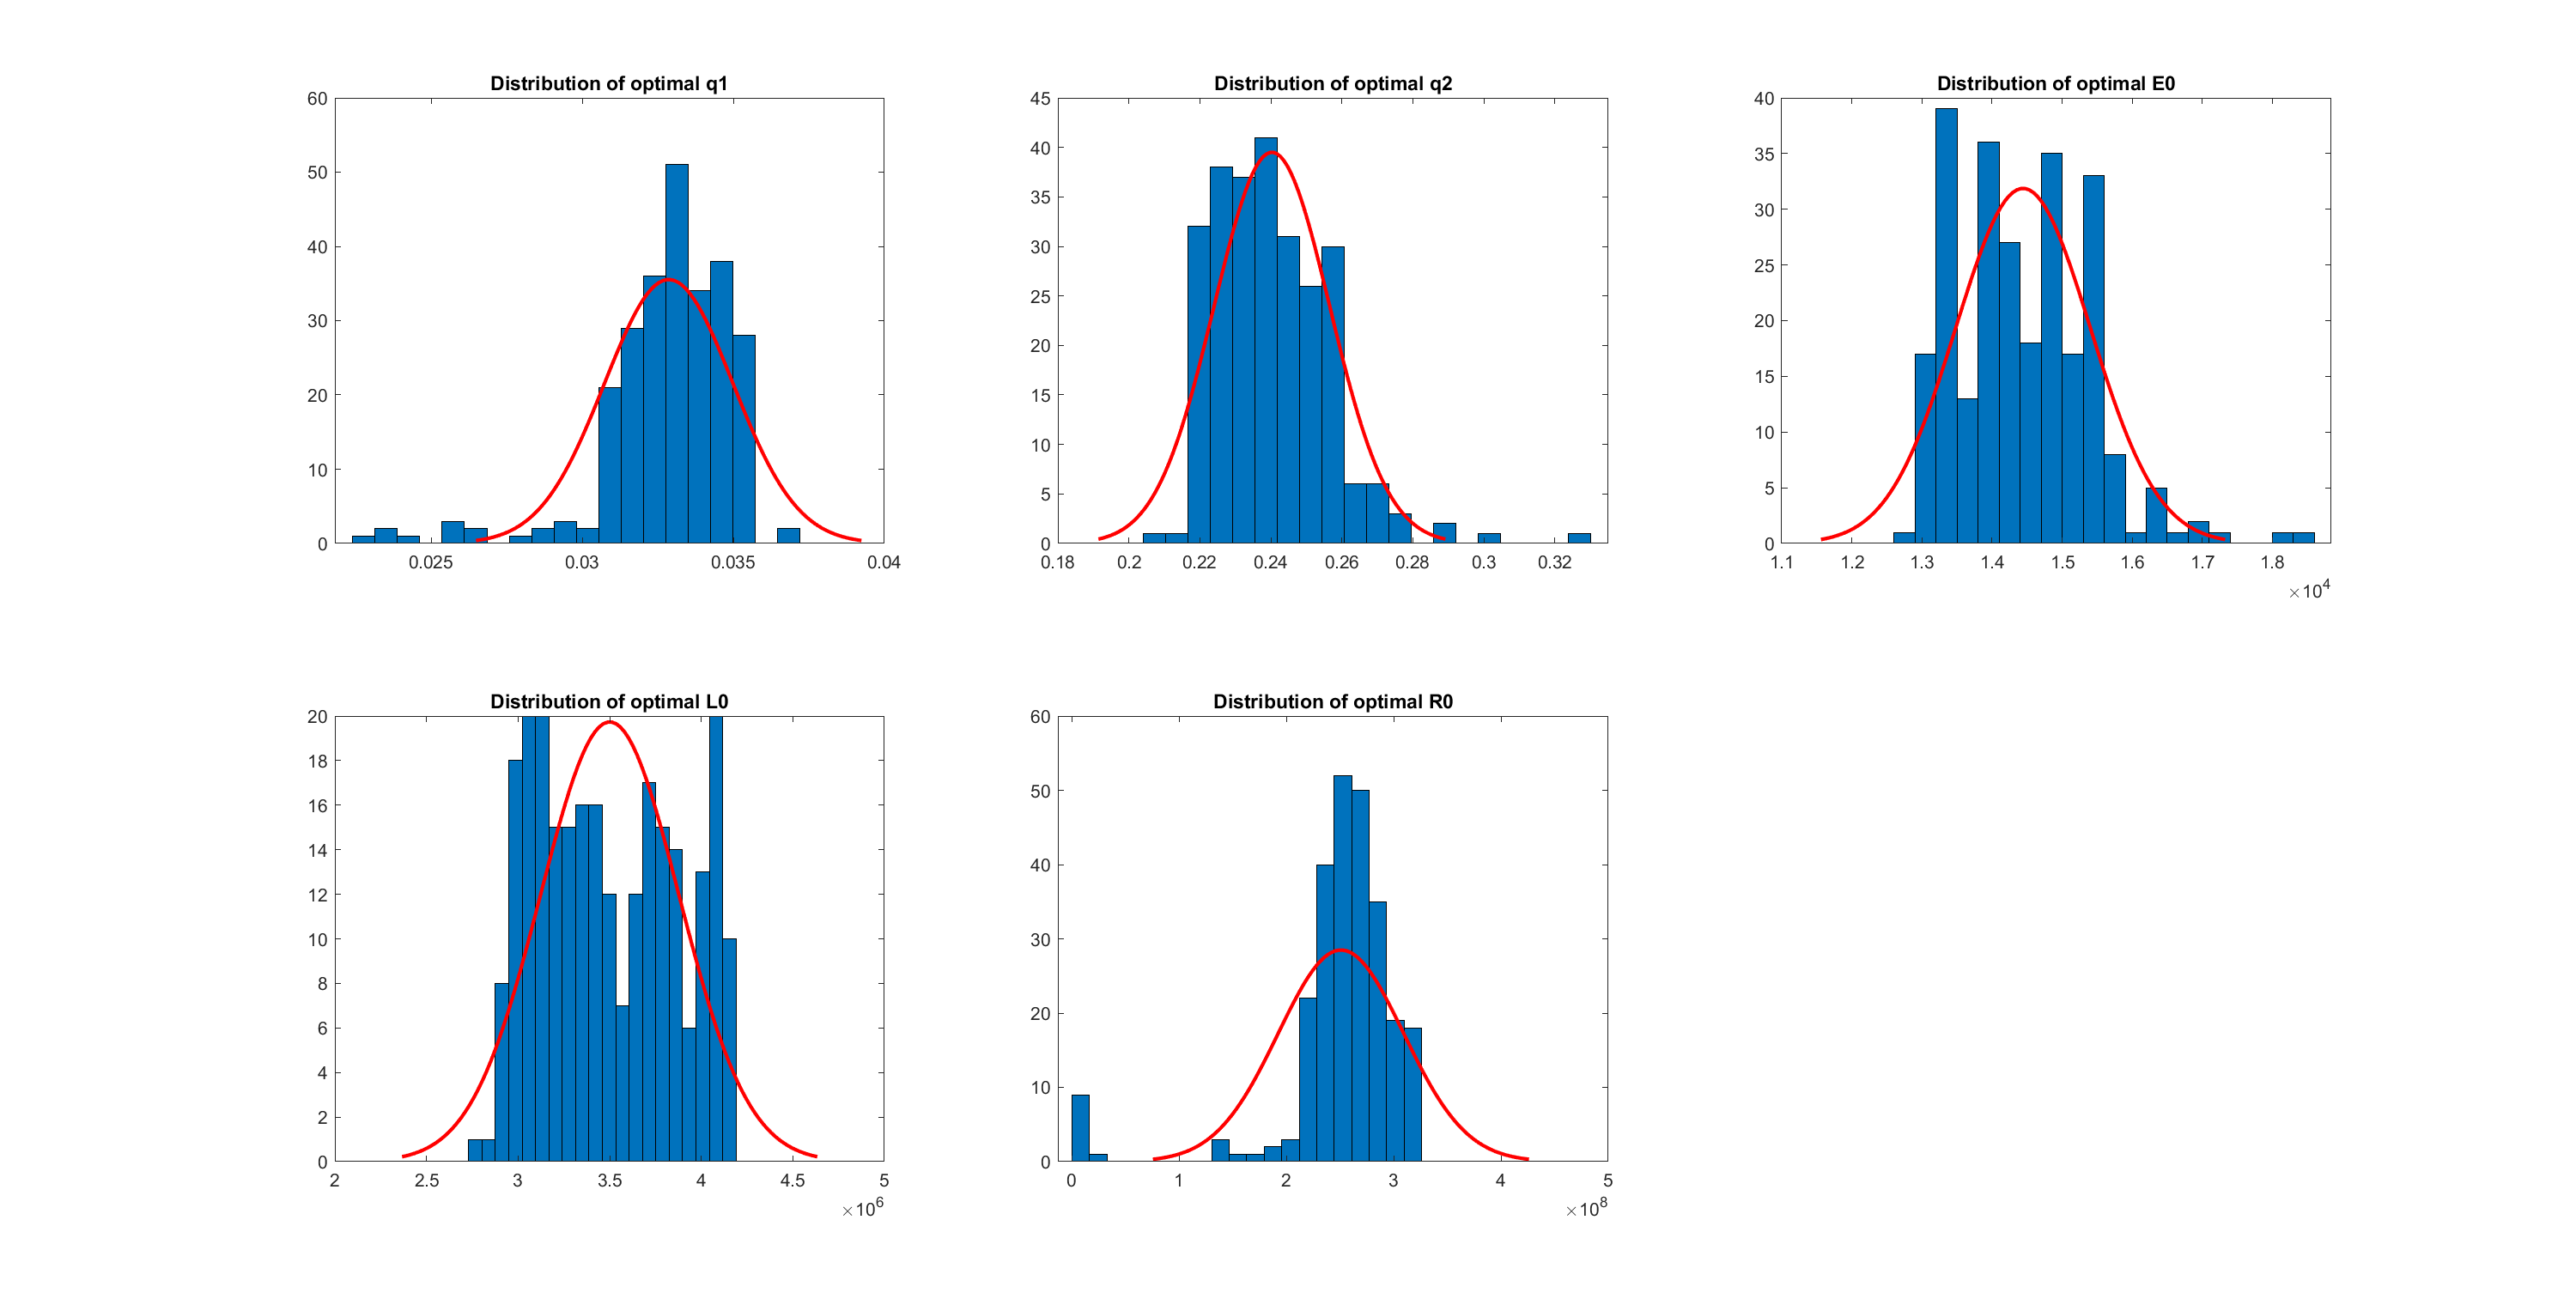
\includegraphics[width=\textwidth]{Optimized parameter distribution across sensitivity analysis Run7Normalization}
	
	\caption{Normalized by scaling (y-ymin)/(ymax-ymin).}
	
	\label{fig:Histo7}
\end{figure}


\section{Future work}

\subsection{Reactivation}
Include an arrow pointing from $R$ to $T$.

Contribution of reinfection to ARI and incidence of TB \cite{Horsburgh2022ContributionDisease}
SEIRE Model\cite{Sulayman2023DynamicsIssues}

Kezia: 
Patients who develop active Tuberculosis more than once in their lifetime can be classified into one of two categories -- exogenous reinfection, or endogenous relapse / reactivation. Cases of relapse are usually linked with drug resistance, commonly found within the first 2 years after treatment ends \cite{Zong2018RelapseChina} \cite{Guerra-Assunção2015RecurrenceFollow-up}. Two Tuberculosis treatment trials conducted in the United States and Canada found that 96\% of recurrent Tuberculosis cases were from reactivation of the initial infecting strain as discussed in \cite{Jasmer2004RecurrentReinfection} . Although some sources claim reinfection is more common than expected \cite{Hoey2002CanTwice}, the proportion of recurrent TB cases due to relapse or reinfection is highly associated with the respective country. Cases of TB reinfection are often linked with the coexistence of HIV \cite{Campbell2022ChapterInfection.}. 

\cite{Brooks-Pollock2011} ``We observed a saturation effect in the number of cases per household and estimated that protective immunity conferred up to 35\% reduction in the risk of disease."

\cite{Mulberry2020} ``the protection afforded to hosts against a new infection from an established one, ... in a population are hard to estimate and cannot be observed directly."  



\subsection{Prevalence}

Data from Canada.  Likelihood?



\section{Introduction}\label{sec1}

We will write this section last

\begin{outline}
    \1 Literature review -- biology of TB, Canadian foreign-born population and screening and immigration (with TB), mathematics 
    \1 Model. Theirs (Guo \& Wu) without any adaptations
        \2 Data
    \1 Show problems with their model: 
        \2 calculate incidence, it's very off [Fig2, top graph]
        \2 $R_0=0$ has problems.
    \1 Optimization using fmincon, their parameters
        \2 $R_0$ same problem
        \2 we include $L_0$ as an optimization (estimated) parameter, but it's extremely dependent on our ``initial choice" of $L_0$.  The optimized $L_0$ stays nearly identical to our initial choice
    \1 Other graphs:
        \2 Sensitivity analysis for $\nu$ and $\omega$ (and many other parameters that don't really matter)
        \2 After sensitivity analysis, we inspect the combinations of parameters that yield low error
        \2 plot error vs (certain) parameter
        \2 post-sensitivity analysis, we have distributions of optimal $q_1,~q_2,~E_0,~ L_0,~ R_0$
        \2 how to pick $L_0$
        \2 (?) updating $L_0$ at every step causes problems in that optimizer no longer changes $E_0$
\end{outline}


\section{The Compartmental Model}\label{sec3}


See \citet{Guo2011PersistentLatency} for a detailed stability analysis of this model.










\backmatter


\bmhead{Acknowledgments}

Support from Langara College - Jeremy and Albert
Support from UM - William



\section*{Declarations}

Some journals require declarations to be submitted in a standardised format. Please check the Instructions for Authors of the journal to which you are submitting to see if you need to complete this section. If yes, your manuscript must contain the following sections under the heading `Declarations':

\begin{itemize}
\item Funding
\item Conflict of interest/Competing interests (check journal-specific guidelines for which heading to use)
\item Ethics approval 
\item Consent to participate
\item Consent for publication
\item Availability of data and materials
\item Code availability 
\item Authors' contributions
\end{itemize}

\noindent
If any of the sections are not relevant to your manuscript, please include the heading and write `Not applicable' for that section. 


%%===========================================================================================%%
%% If you are submitting to one of the Nature Portfolio journals, using the eJP submission   %%
%% system, please include the references within the manuscript file itself. You may do this  %%
%% by copying the reference list from your .bbl file, paste it into the main manuscript .tex %%
%% file, and delete the associated \verb+\bibliography+ commands.                            %%
%%===========================================================================================%%

\bibliography{TB-references,more}

\end{document}
